\documentclass[11pt,a4paper]{article}
\usepackage[table,xcdraw]{xcolor}
\usepackage[portuguese]{babel}
\usepackage[utf8]{inputenc}
\usepackage{graphicx}
\usepackage{float}
\usepackage{indentfirst}
\usepackage{hyperref}
\usepackage{makecell}
\usepackage[toc,title]{appendix}
\usepackage{a4wide}
\usepackage[official]{eurosym}

\renewcommand{\appendixtocname}{Ap\^endices}
\renewcommand{\appendixpagename}{Ap\^endices}

\newcommand{\requirement}[3]{
    #1 (#3)
}

\begin{document}

\setcounter{tocdepth}{4}
\setcounter{secnumdepth}{4}
\begin{titlepage}

\newcommand{\HRule}{\rule{\linewidth}{0.5mm}} % Defines a new command for the horizontal lines, change thickness here

\center % Center everything on the page

\begin{figure}[H]
    \centering
    
\includegraphics[scale=0.5]{images/UM_EENG.jpg}
    \label{figUM}
\end{figure}

\large Universidade do Minho\\[0.2cm] % Name of your university/college
\large Mestrado Integrado em Engenharia Informática\\[0.2cm] % Major heading such as course 
\large Departamento de Informática\\[2.5cm] % Major heading such as course name

\textsc{\Large Projeto em Engenharia Informática}\\[0.3cm] % Minor heading such as course title
\HRule \\[0.3cm]
{ \LARGE \bfseries Automação Robótica de Processos (RPA) usando um chatbot Telegram}\\[0.3cm] % Title of your document
\HRule \\[0.3cm]

\begin{figure}[H]
    \centering
    
\includegraphics[scale=0.6]{images/nos.png}
    \label{figNOS}
\end{figure}

% [2.5cm]

{\large Ano Letivo de 2019/2020}\\ % Date, change the \today to a set date if you want to be precise

\vspace*{\fill}
\noindent
{\large \textbf{Grupo i1}}\\[0.5cm]
Fábio Gonçalves \textsc{A78793}\\[0.3cm]
Francisco Oliveira \textsc{A78416}\\[0.3cm]
Gonçalo Camaz \textsc{A76861}\\[0.3cm]
João Vieira \textsc{A78468}\\[0.3cm]
José Carlos Martins \textsc{A78821}\\[0.3cm]
Miguel Quaresma \textsc{A77049}\\[0.3cm]
Raul Vilas Boas \textsc{A79617}\\[0.3cm]
Salete Teixeira \textsc{A75281}\\[0.3cm]
Simão Barbosa \textsc{A77689}

\end{titlepage}

\newpage

\thispagestyle{empty}
\setcounter{page}{0}
\tableofcontents
\clearpage

\newpage

\section{Introdução}
\subsection{Propósito do sistema}
Atualmente, fornecedores de serviço como a NOS estão "presentes" em casa da maioria dos portugueses,
disponibilizando serviços como pacotes de televisão, \textit{internet}, telefone e tarifários móveis.  A
diversidade destes serviços tem aumentado exponencialmente, bem como a sua qualidade, observando-se ainda
uma interação entre os mesmos que leva à existência de sistemas mais complexos.  Apesar da clara
conveniência que estes sistemas providenciam, a complexidade exigida pelos mesmos propicia a ocorrência de
problemas/falhas técnicas, que não são de trivial resolução para um utilizador normal. Como tal, para que a
qualidade do serviço não sofra em detrimento da sua complexidade, torna-se necessário o estabelecimento de
sistemas de apoio ao cliente que facilitem a resolução de problemas técnicos, minimizando o
\textit{downtime} do serviço.  Nesse sentido, a automação robótica de processos usando um \textit{chatbot}
permitirá aumentar a capacidade de atendimento da NOS para resolução de problemas técnicos ao eliminar as
limitações inerentes à mão de obra humana. Isto traduzir-se-á numa redução nos tempos de espera por
assistência e nos tempos de resposta e num aumento no número de clientes que podem ser atendidos em
simultâneo.  Adicionalmente, o desenvolvimento de um \textit{chatbot} que integre outras vertentes dos
serviços disponibilizados pela NOS, como cinemas e tarifários móveis, permitirá o esclarecimento de dúvidas
que digam respeito aos mesmos. Isto resulta numa maior facilidade de acesso à informação que, de outra
forma, estaria distribuída por diversos \textit{websites}, dificultando a sua consulta.


\subsection{Cliente, consumidores, parte interessadas}

Tendo em conta a aplicação que se desenvolveu, podemos considerar que existem várias partes
interessadas, e, apesar de nem todas terem a mesma importância no estudo realizado, todas devem ser tidas em
conta de forma a melhorar o trabalho desenvolvido. Desta forma, podemos dividir as partes interessadas em
quatro categorias: cliente, utilizadores, compradores e outras partes interessadas.

\begin{itemize}
    \item \textbf{Cliente}\newline
    O cliente deste sistema é a empresa \textbf{NOS}, que pretende que seja desenvolvido o sistema descrito
    de forma a poder ser fornecido aos seus clientes, como forma de resolução de problemas, e também com o
    intuito de captar novos clientes, quer seja pela disponibilização de informações dos seus serviços (como
    tarifários, telemóveis, etc) ou dos seus cinemas. A introdução de um sistema como este numa companhia da
    dimensão da NOS pode não só levar a uma maior captação de possíveis clientes e consequente entrada de
    valores financeiros, como possivelmente reduzir no número de funcionários responsáveis pela parte de
    \emph{call-center}.
    \item \textbf{Utilizadores}\newline
    Os utilizadores do sistema em questão são os clientes da NOS (motivados pela resolução de problemas
    técnicos associados ao serviço NOS e esclarecimento de dúvidas dos serviços NOS), dos cinemas da NOS
    (pretendem consultar informação relativa à exibição de filmes nos cinemas NOS), ou clientes
    de outros fornecedores de serviço (pretendem consultar os serviços da NOS por forma a averiguar se 
    adequam às suas necessidades). Todos os tipos de utilizadores devem ser tidos em conta, visto que são os
    mesmos a dar uso à aplicação, e o sucesso da mesma depende destes. O papel dos clientes dos cinemas da NOS
    pode ser desempenhado pelos outros dois utilizadores.
    \item \textbf{Compradores}\newline
    Os compradores deste sistema é o mesmo grupo de pessoas que compõe os utilizadores. São as pessoas que adquirem o sistema assim que o mesmo esteja disponível
    para comercialização (mesmo não estando envolvida necessariamente uma transação financeira).
    \item \textbf{Outras partes interessadas}\newline
    Podemos considerar outras partes interessadas que podem ser identificadas no desenvolvimento de um
    sistema como o descrito, tais como:
    \begin{itemize}
        \item Possíveis empresas concorrentes da NOS, que devem ter interesse em verificar se uma solução
        como esta pode ser vantajosa de incluir na sua empresa.
        \item o próprio \emph{Telegram}, plataforma através do qual é feito o contacto com os compradores do
        sistema.
        \item Empresas/Projetos que desenvolvam sistemas semelhantes (\emph{chatbot's}, inteligência
        artificial, processamento de linguagem, etc)
    \end{itemize}
    
\end{itemize}

\subsection{Convenções de Nomenclatura e Definições}
\subsubsection{Definições}
\begin{itemize}
    \item \textit{Web Scraping}: Processo automático de extração de dados de \textit{websites}.
    \item \textit{ChatBot}: Comunicação entre uma ``máquina'' e um utilizador.
    \item \textit{Messaging}: Envio de mensagens.
\end{itemize}
\subsubsection{Dicionário de Dados}
\begin{itemize}
    \item \textbf{Problema técnico:} problema relacionado com serviços oferecidos pela NOS.
    \item \textbf{Sessão:} exibição de um filme num determinado horário e cinema.
\end{itemize}

\subsection{Âmbito do Sistema}
O diagrama de \textit{use cases} de seguida apresentado serve o propósito de indicar quais os 
actores do sistema desenvolvido bem como as ações que cada um pode tomar, sendo estas limitadas
pelas funcionalidades disponibilizadas pelo sistema.
\begin{figure}[H]
    \centering
    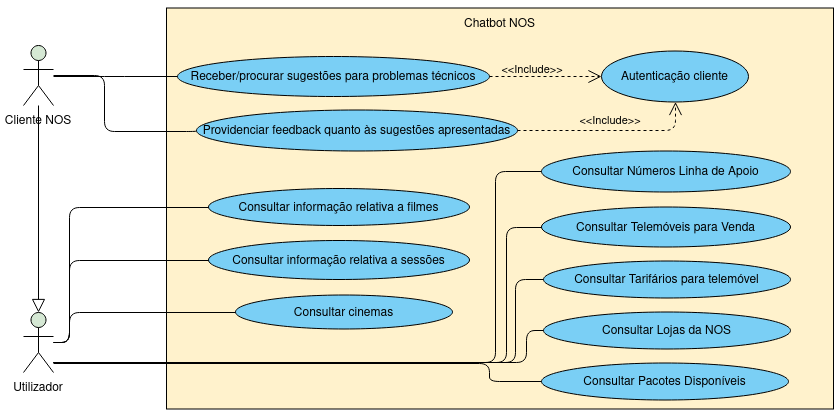
\includegraphics[width=13cm]{images/usecases_model.png}
    \caption{Diagrama de \textit{use cases} do sistema}
    \label{fig:use_case_diag}
\end{figure}

A distinção entre Cliente NOS e Utilizador deve-se ao facto de certos serviços, como a resolução
de problemas técnicos, serem interditos a utilizadores que não sejam clientes da NOS. No entanto,
utilizadores nesta condição têm permissão para consultar informação relativa a cinemas NOS ou mesmo
aos serviços por esta providenciados, tornando-os potenciais clientes.

\section{Distribuição de Tarefas}

O período de desenvolvimento do sistema, de 29 de setembro a 24 de janeiro (aproximadamente 16 semanas), foi
dividido em \textit{sprints} de duas semanas, seguindo a metodologia de desenvolvimento \textit{Agile}. 
Por forma a facilitar a distribuição de tarefas, o grupo organizou-se em 3 equipas de 3 elementos,
cada uma responsável por cumprir um conjunto de objetivos em cada \textit{sprint}, sendo 
as equipas atribuídas às tarefas tendo em conta os perfis de especialização dos seus membros.
No fim de cada \textit{sprint} foram realizadas reuniões por forma a serem definidos os objetivos para o 
\textit{sprint} seguinte.
De seguida estão apresentadas as 3 equipas e tarefas atribuídas a cada uma delas:

\begin{table}[H]
    \centering
    \footnotesize
    \begin{tabular}{| c | c |}
        \hline
        Equipa & Tarefas \\ \hline
        \makecell{Francisco Oliveira\\ José Martins\\ Raúl Vilas Boas} & \makecell{Chat Processor \\ Telegram API Endpoint} \\ \hline
        \makecell{João Vieira\\ Miguel Quaresma\\ Simão Barbosa} & \makecell{Cinemas Webscraper \\ Resolução de Problemas \\ Telegram API Endpoint} \\ \hline
        \makecell{Salete Teixeira\\ Gonçalo Camaz\\ Fábio Gonçalves} & \makecell{FS Webscraper \\ Modo regras do Chat Processor} \\ \hline
    \end{tabular}
    \caption{Distribuição das tarefas pelas equipas}
\end{table}

Apesar desta distribuição de tarefas, nos últimos \textit{sprints} houve uma interajuda entre as equipas,
pelo que as tarefas definidas para as últimas semanas tiveram o envolvimento de membros de diferentes
equipas.

\section{Recursos Necessários}
O desenvolvimento de projetos de engenharia software complexos exige a utilização de recursos tecnológicos
que permitam não só facilitar a implementação do sistema, mas também a gestão da equipa de
desenvolvimento. Nesse sentido, a gestão do grupo, nomeadamente na distribuição de tarefas e ``controlo'' de
\textit{sprints}, foi realizada com recurso à ferramenta \textit{Trello}, que permitiu decompor o processo
de desenvolvimento em diferentes fases e manter um registo do número, e estado, das tarefas existentes. No
que diz respeito à implementação, e para facilitar a colaboração entre os diversos elementos bem como a
gestão das diferentes modificações do código de cada componente, foi usado o sistema de controlo de versões
e trabalho cooperativo \textit{Git}. Por fim, na \textit{stack} de tecnologias utilizada, a infraestrutura
do projeto foi implementada recorrendo a \textit{frameworks} como \textit{Flask} e \textit{Django} para a
implementação de servidores HTTP, \textit{SQLite} como sistema de gestão de base de dados, \textit{Redis}
para permitir o uso de \textit{in-memory cache} e \textit{Docker} para o \textit{deployment} do sistema
final. A linguagem escolhida, \textit{Python}, permitiu ainda o uso do vasto número de módulos existente
de entre os quais modelos para processamento de linguagem natural e reconhecimento de entidades como
\textit{deeppavlov} baseado no \textit{BERT}. A interação com o utilizador, através da aplicação
\textit{Telegram}, exigiu o acesso à API desta mesma aplicação\footnote{Ver
\url{https://core.telegram.org/bots/api}}.

\section{Implementação}

\subsection{Arquitetura}
O desenvolvimento de aplicações escaláveis e complexas pressupõe que os seus componentes possam ser
desenvolvidos de forma isolada, desde que as \textit{interfaces} de cada um, que permitem a interação com o
exterior (\textbf{i.e.} APIs), sejam previamente definidas. Isto permite que os detalhes da implementação
de um determinado componente sejam transparentes aos restantes componentes do sistema. Nesse sentido, o
presente sistema foi desenvolvido seguindo uma arquitetura de microserviços, em que cada serviço tem
funcionalidades claramente definidas que expõe através da sua API. O seguinte diagrama permite observar a
interação entre os diferentes componentes do sistema:

\begin{figure}[H]
    \centering
    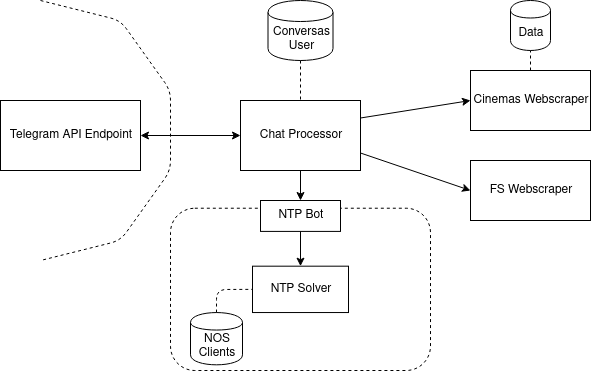
\includegraphics[width=10cm]{images/arch.png}
    \caption{Arquitetura do sistema}
    \label{fig:arch}
\end{figure}

Como é possível observar, os componentes encontram-se divididos tendo em conta o tipo de serviço que
providenciam: informação sobre cinemas (\textit{Cinemas Webscraper}), serviços da NOS (\textit{FS Webscraper}), resolução
de problemas (\textit{NTP Bot} e \textit{NTP Solver}), processamento de linguagem natural (\textit{Chat
Processor}) e interação com o serviço de \textit{messaging} (\textit{Telegram API Endpoint}). No sistema
desenvolvido, e como será referido nas secções seguintes, o componente \textit{Telegram API Endpoint} é
responsável pela interação com a API do \textit{Telegram}. Uma das características destes sistema diz
respeito à independência do mesmo relativamente ao serviço de \textit{messaging} escolhido, o que permite
que este seja alterado sem ser necessário modificar nenhum microserviço para além do responsável pela
interação com a respetiva API, que deverá respeitar a API definida pelo sistema para este serviço. No
entanto, o ponto de entrada no sistema corresponde ao \textit{Chat Processor}, que é responsável por
interpretar as mensagens dos utilizadores e responder em conformidade. Assim sendo, a sua função é a de
delegar ``tarefas'' pelos restantes componentes que, tal como no caso do serviço de \textit{messaging},
podem ser alterados desde que respeitem a API para eles definida, mediando a interação entre estes e o
utilizador. A funcionalidade de cada um destes clientes será tornada mais evidente nas próximas secções.


\subsection{Telegram API Endpoint}
Este componente pode ser considerado como o ponto de entrada e saída de mensagens no sistema, funcionando
como intermediário entre a aplicação de \textit{messaging}, Telegram neste caso, com a qual comunica através
da respetiva API, e o \textit{bot} em si. Ou seja, as mensagens que são enviadas para o \textit{bot} são
recebidas primeiramente neste serviço, sendo depois enviadas para o \textit{Chat Processor} que trata de interpretar
as mesmas e, quando tem uma resposta pronta para enviar ao utilizador, trata de invocar novamente este
serviço para enviar a mensagem.

Uma das propriedades fundamentais deste componente diz respeito à sua modularidade, isto é, se num futuro
for necessário alterar ou acrescentar um serviço de \emph{messaging} (Whatsapp, Messenger, etc) distinto,
que faça uso de todos os outros componentes do sistema, apenas bastará que esse trate de interagir com a API
desse mesmo serviço de mensagens e que implemente os \emph{endpoints} que este componente expõe, de forma
que o número de alterações a efetuar no sistema seja mínimo.

Alguns dos \emph{endpoints} implementados que permitem uma maior interação com o utilizador do \textit{bot} 
são:

\begin{itemize}
    \item \texttt{POST /send\_message} - permite que o sistema envie mensagens para o utilizador.
    \item \texttt{POST /send\_silent\_message} - permite fazer o envio de mensagens sem que o utilizador
      receba o som de uma notificação. Este método é utilizado para enviar mensagens para os utilizadores
      inativos, como mais à frente é explicado.
    \item \texttt{POST /send\_photo} - permite enviar fotos com uma legenda, o que permite uma melhor
      visualização e experiência de utilização com o Bot.
    \item \texttt{POST /get\_location} - permite pedir ao utilizador a sua localização, que pode ser
      utilizada em pedidos de informações efetuados pelo mesmo.
    \item \texttt{POST /send\_keyboard} - permite enviar menus para o utilizador, sendo este método utilizado
      para um modo interativo que mais à frente é mencionado.
\end{itemize}

Para além destes métodos que foram desenvolvidos para serem compatíveis com outros serviços de
\textit{messaging}, no caso deste componente que usa especificamente a API do Telegram, é ainda implementado
um \emph{endpoint} \texttt{/webhook} para o qual o Telegram fica encarregue de enviar atualizações
(mensagens) do \textit{bot}. Isto porque quando executados este componente a primeira tarefa que ele executa
é ``dizer'' ao Telegram através do método \texttt{/setWebhook} da sua API qual o \emph{url} para o qual deve
enviar atualizações do \textit{bot}, que no nosso caso será um \emph{url} disponibilizado pela ferramenta
\texttt{ngrok} mais o \emph{endpoint} \texttt{/webhook}.


\subsection{Chat Processor}
O \textit{Chat Processor} é a componente central do sistema no que diz respeito a controlar as várias interações com
os utilizadores. Este componente recebe as mensagens enviadas pelo utilizador (encaminhadas pelo Telegram
API Endpoint) e categoriza-as de forma a determinar o que o utilizador pretende, que determinará a resposta
dada ao utilizador. Esta resposta pode tomar várias formas: uma questão ao utilizador, os resultados finais
a apresentar, um menu com botões (referente ao modo interativo/regras), uma mensagem (de erro) a indicar que
não foi possível obter a informação pretendida ou que não foi possível atribuir uma categoria à mensagem do
mesmo.

Os 3 modos de funcionamento distintos deste componente alteram consideravelmente a sua resposta a mensagens
do utilizador. Quando a mensagem do utilizador é recebida, o sistema tenta determinar, com recurso a
expressões regulares, se o que o utilizador pretende é um dos seguintes comandos:
\begin{itemize}
    \item \texttt{/start}: informação inicial acerca do Bot
    \item \texttt{/help}: informação adicional acerca do Bot
    \item \texttt{/reset}: permite reiniciar a conversa que o utilizador tem com o Bot. Realiza o
      \textit{reset} do estado da conversa.
\end{itemize}

De seguida, e visto que o utilizador pode ter requisitado informação acerca de cinemas onde, por vezes, a
informação obtida do \textit{Cinemas Webscraper} possui mais do que um cinema, verifica-se se a mensagem do
utilizador é a indicação de que cinema pretende dos que lhe foram apresentados, devolvendo então ao
utilizador a informação pretendida para esse cinema. No caso de haver apenas um cinema a informação é logo
apresentada.

Caso contrário, obtém-se da base de dados (Redis) o estado atual da conversa com o utilizador. Após este
passo, verifica-se se a mensagem enviada pelo utilizador tem como objetivo enviar a sua localização e, se
assim for, é guardada essa mesma informação no estado da conversa.

No seguimento deste fluxo, verifica-se em que estado se encontra a conversa, visto que o mesmo determinará
qual a ação seguinte. Caso o estado seja ``modo regras'', então a mensagem do utilizador é encaminhada para
esse modo e, caso o estado seja ``modo problemas'' a mensagem é também encaminhada, mas para o componente
NTP Bot (Resolução de Problemas). Caso o estado da conversa não seja nenhum destes dois verifica-se,
recorrendo de novo a expressões regulares, se a mensagem corresponde a um dos seguintes comandos:

\begin{itemize}
    \item \texttt{/interativo} ou \texttt{modo regras}, ou ainda \texttt{modo de regras}: modo interativo
      que pretende facilitar a interação que o utilizador tem com o Bot. Este modo será aprofundado na
      secção~\ref{sec:modoregras}. O estado da conversa passa a ser "modo regras".
    \item \texttt{/mais} ou \texttt{ver mais}: Quando uma resposta a devolver ao utilizador é uma lista e
      possui mais de cinco elementos são apresentados apenas os primeiros cinco e, com recurso a este comando, é
      possível obter os próximos cinco, evitando sobrecarregar a conversa com informação.
\end{itemize}

Se a mensagem enviada não corresponder a nenhum destes comandos, dá-se início ao processo de categorização
da mesma, com base nos três serviços disponibilizados pelo \textit{bot}, e tendo em conta o estado atual da
conversa.

É então verificado se o utilizador se encontra no estado de "mudar categoria?", ou seja, o utilizador foi
questionado se pretende mudar de assunto na conversa, por exemplo, se pretende deixar de conversar sobre
telemóveis e passar a conversar sobre cinemas. Caso pretenda alterar o assunto, o estado da conversa atual
é parcialmente limpo, por exemplo, horas, datas que já tinha dito e que já tinham sido interpretadas. Por
outro lado, caso pretenda continuar no mesmo estado, a mensagem que desencadeou a mudança de assunto é
processada de modo a detetar entidades e parâmetros presentes na mensagem que possam ser relevantes para
o assunto atual.

Caso o estado não seja de "mudar categoria?" o objetivo passa por detetar a funcionalidade a que o
utilizador pretende aceder. A cada uma destas funcionalidades estão associadas informações como o URL a
utilizar, as palavras (expressões regulares e o seu peso) usados na deteção da funcionalidade e os parâmetros
(opcionais e obrigatórios) que a mesma recebe. A categorização da mensagem consiste em somar os pesos das
palavras de cada funcionalidade que aparecem na mensagem introduzida pelo utilizador, sendo escolhida a
funcionalidade cuja confiança for a mais elevada. Caso este valor seja inferior a 0.7, então não se
considera a funcionalidade detetada e o utilizador é avisado de que não foi possível perceber o pretendido. É
importante realçar que, previamente ao cálculo desta confiança, a mensagem é processada por forma a remover
erros ortográficos, acentos e pontuação, sendo ainda convertida para caracteres minúsculos. A correção
ortográfica é realizada através da biblioteca \texttt{symspellpy}, que usa o algoritmo \texttt{SymSpell}\footnote{Ver \url{https://github.com/wolfgarbe/symspell}}. O uso deste algoritmo pressupõe a existência de
um ficheiro com as palavras mais frequentes, beneficiando ainda de um outro ficheiro com os bi-grams (duas)
mais frequentes na língua portuguesa. A qualidade da correção é diretamente influenciada pela qualidade
destes dois \textit{datasets}, que foram criados com recurso a um \textit{corpus} \textit{OpenSubtitles}
disponível em \url{http://opus.nlpl.eu/OpenSubtitles-v2018.php}.

Caso a funcionalidade pretendida não seja detetada, com confiança suficiente, após 5 mensagens consecutivas,
é enviada ao utilizador uma mensagem que sugere o recurso a alternativas como o modo regras ou as linhas de
apoio da NOS.

Após a deteção da funcionalidade com a confiança necessária e, caso a funcionalidade detetada seja a de
resolução de problemas (\texttt{/solver}), então a mensagem do utilizador é reencaminhada para o NTP Bot e o
estado da conversa passa para "modo problemas".  Caso contrário, ou seja, caso a funcionalidade detetada não
seja de resolução de problemas, a fase seguinte passa por determinar os parâmetros que a funcionalidade
precisa, sejam estes opcionais ou obrigatórios, tendo em conta que alguns já possam estar presentes na
mensagem. Dada a sua natureza, os parâmetros obrigatórios que ainda não tenham sido obtidos, são
requisitados ao utilizador. No caso de não faltar nenhum destes parâmetros, o resultado é apresentado ao
utilizador. Nos casos em que o número de parâmetros opcionais por preencher seja superior a um determinado
valor, é enviado ao utilizador um conjunto de resultados preliminares que podem ser posteriormente filtrados
com base nos parâmetros opcionais, caso este assim o deseje.

Um dos parâmetros obrigatórios, que está presente em diversas funcionalidades, corresponde a uma localização
que é do interesse do utilizador. Podendo representar locais onde pretende consultar a existência de cinemas
ou a localização atual do mesmo, quando necessite de se deslocar à loja NOS mais próxima. Nas
funcionalidades em que este parâmetro é necessário, o utilizador pode responder de duas formas, fornecendo a
sua localização GPS através do botão presente no Telegram, ou pode indicando, por escrito, uma cidade ou
município. Caso não seja possível determinar a localização indicada pelo utilizador, é realizada uma
segunda tentativa no que diz respeito a determinar a localização em causa.

Para além dos parâmetros obrigatórios existe ainda uma situação particular em que uma funcionalidade
apresenta apenas parâmetros opcionais sendo, no entanto, obrigatória a presença de pelo menos um destes.
Nestes casos o utilizador pode indicar qualquer um dos parâmetros opcionais referidos, sendo-lhe apenas
exigido que indique pelo menos um.

As perguntas sobre parâmetros opcionais dão a indicação, ao utilizador, de que não necessita de responder,
podendo dizer "Não" ou uma variante deste (com letras maiúsculas/minúsculas ou sem acento, etc) para que o
parâmetro seja ignorado. Em casos em que o utilizador indique um valor que não corresponde a "Não", as
entidades presentes na mensagem são identificadas, no sentido de encontrar associações com os parâmetros em
causa. Em último recurso, e caso não seja identificada nenhuma entidade, assume-se a mensagem do utilizador
como o valor do parâmetro a usar.

Existem ainda alguns parâmetros opcionais especiais, parâmetros ``booleanos'', em que o seu valor só pode
ser "Sim" ou "Não". Nestes casos, os valores possíveis são indicados ao utilizador e, caso o mesmo não
responda com um destes valores (ou uma das suas variantes), é realizada uma nova tentativa com a mesma
pergunta.

Os parâmetros já detetados e os que ainda estão em falta (ou seja que ainda não foram
fornecidos pelo utilizador) são mantidos no estado da conversa do utilizador.

Como já referido, as frases dos utilizadores são utilizadas num processo de deteção de entidades que permite
extrair valores para os parâmetros que cada funcionalidade possui. Para que isto seja possível, cada
parâmetro é associado a um tipo de entidade que será detetado no processo mencionado. A deteção de entidades
é conseguida com recurso a duas abordagens distintas que são executadas de maneira sequencial/composta:

\begin{itemize}
    \item Modelo NER (Named Entity Recognition) multilíngua do \texttt{deeppavlov}\footnote{Ver
        \url{https://demo.deeppavlov.ai/\#/mu/ner} e
        \url{http://docs.deeppavlov.ai/en/master/features/models/ner.html}}: Modelo baseado no modelo
      BERT\footnote{Ver \url{https://github.com/google-research/bert}} e pré-treinado com o corpus Ontonotes.
      Deteta cerca de 18 entidades diferentes, sendo que destas apenas nos importam nomes (\texttt{PERSON}),
      locais (\texttt{GPE}), marcas (\texttt{PRODUCT}), filmes (\texttt{WORK OF ART}), datas (\texttt{DATE}),
      horas (\texttt{TIME}), quantidades monetárias (\texttt{MONEY} ou \texttt{CARDINAL}) e números
      (\texttt{CARDINAL}). Apesar de já detetar grande parte das entidades necessárias, não deteta todas as que
      necessitamos para além de que por vezes não deteta corretamente entidades que é necessário detetar.  Por
      tais razões foi implementado a abordagem do ponto seguinte.  Foi também implementado uma \textit{blacklist},
      com o intuito de ignorar entidades detetadas pelo modelo visto que por vezes o modelo deteta um dos
      comandos já especificados como, por exemplo, uma entidade do tipo \texttt{PERSON}.
    \item Reconhecimento de entidades através de expressões regulares: deteta as entidades presentes na
      mensagem através de expressões regulares a partir de um conjunto de tuplos com palavra(s) e o tipo de
      entidade a associar. Portanto de uma forma simples quando a palavra ou palavras são encontradas na mensagem
      são assumidas como uma entidade do tipo associado a esta(s) palavra(s).  Por forma a isto funcionar em casos como filmes,
      marcas de telemóveis, modelos de telemóveis, tarifários e assuntos da linhas de apoio é necessário obter as
      possíveis palavras dos \textit{scrapers} (Cinema e FS).  Para tal é realizado em \textit{background} um
      \textit{update} de uma em uma hora requisitando esta informação aos \textit{scrapers}.  Para além destas, são também
      detetados neste modo, todos os municípios portugueses (foi criado um ficheiro com a informação destes),
      tipos de pacotes, os possíveis serviços de um pacote, géneros de filmes, moradas e expressões como
      ``amanhã'', ``hoje'', ``manhã'', ``tarde'' e ``noite''.
\end{itemize}

Após a deteção das entidades, e nos casos em que seja aplicável, é necessário converter os valores para os
formatos esperados pelos \textit{endpoints} correspondentes. Estes casos correspondem a entidades do tipo
data, horas, valores monetários ou numéricos. Como tal, datas escritas por extenso (\textbf{e.g.} 21 de
janeiro) ou numa forma mais compacta (\textbf{e.g.} 21/1/2020) são convertidas para o formato ``YYYY-MM-DD''
(\textbf{e.g.} 2020-01-21). Uma particularidade desta conversão diz respeito à capacidade de converter
indicadores temporais relativos \textbf{i.e.}  ``hoje'' e ``amanhã'' são convertidos para a data atual e do
dia seguinte, respetivamente. No caso de horas, tanto em extenso (\textbf{e.g.}. 21 horas e 10 minutos) ou
na sua forma compacta (\textbf{e.g.} 21h10 ou 21:10) o formato alvo corresponde a ``HH:MM:SS''
(\textbf{e.g.} 21:10:00). Nos casos em que estes valores digam respeito a intervalos de tempo, expressões
como ``manhã'', ``tarde'' e ``noite'' são convertidas em duas horas distintas que representem o período
correspondente. No caso dos valores numéricos, a representação alvo corresponde à sua representação através
dos algarismos constituintes (\textbf{e.g.} ``vinte e um'' $\mapsto$ 21). No caso de valores monetários o
processo é semelhante, sendo apenas necessário remover a palavra ``euros'' ou o respetivo símbolo
(\euro{}).

O processo de associação entre entidades e os respetivos parâmetros é feito, na maioria dos casos através da
comparação do tipo da entidade obtida com o tipo(s) da entidade associada ao parâmetro. Contudo, existem três
casos excecionais em que dois parâmetros de uma mesma funcionalidade necessitam do mesmo tipo de
entidade. Estes casos são valores mínimos e máximos (\textit{min} e \textit{max}), intervalos de tempo
(\textit{start\_time} e \textit{end\_time}) ou nomes próprios (\textit{cast} e \textit{producer}). Nestes
casos, o mapeamento nos parâmetros é feitos de forma progressiva, escolhendo primeiro um dos parâmetros
possíveis (\textit{min}, \textit{start\_time}, \textit{cast}) e de seguida os restantes.

Quando todos os parâmetros estão preenchidos, ou caso o utilizador utilize o comando \texttt{/mostrar} (ou
\texttt{mostrar resultados}) quando é questionado por um parâmetro opcional é apresentada ao utilizador a
informação que corresponde aos parâmetros inseridos. Esta informação é obtida a partir dos componentes
\textit{Cinemas Webscraper} e \textit{FS Webscraper}, sendo formatada textualmente (\textit{pretty print}) com o intuito de
facilitar a sua leitura por parte do utilizador.

Por fim, é importante referir que quando o utilizador se encontrar inativo por mais de 5 minutos, é-lhe
enviada uma mensagem \textit{silenciosa} com indicação dos comandos suportados pelo \textit{bot},
facilitando futuras interações com o mesmo. Para além desta mensagem, o contexto da interação com o
utilizador é removido, de forma semelhante ao que acontece com o comando \texttt{/reset}, evitando assim que
o utilizador esteja a meio de uma conversa com o \textit{bot} da qual já não se recorda. A implementação
desta tarefa surge de discussões com a empresa.

\subsubsection{Modo de Regras}\label{sec:modoregras}

Tal como referido anteriormente, o modo de regras foi desenvolvido para providenciar uma utilização
orientada através de botões. Esta interação foi criada com o intuito de auxiliar os utilizadores que não
possuem conhecimentos relativos ao funcionamento do bot. Este modo permite assim aos utilizadores obter
informações relativas aos serviços providenciados pela NOS, descritos na secção~\ref{sec:fs_scrapper}, como
também informações sobre os cinemas, descritos na secção~\ref{sec:cinemas}. Caso o utilizador pretenda o
modo de resolução de problemas, é reencaminhado para o modo de resoluções técnicas, descrito na
secção~\ref{sec:resTec}. Para uma melhor perceção do fluxo de atividades do modo de regras, podem ser
consultados os diagramas disponíveis no anexo~\ref{anexo1}.

Para melhorar a usabilidade do modo de regras, tirou-se proveito dos menus de opções através de botões, os
\textit{keyboards}, disponibilizados pelo \textit{Telegram}. Assim, através de cliques, o utilizador pode
navegar pelo mesmo, com uma interface semelhante à demonstrada na Figura \ref{fig:figModoRegras}. Caso sejam
necessários inputs por parte do utilizador, o bot apresenta uma mensagem a descrever o que pretende receber,
como por exemplo, o preço de algum serviço ou o nome de um filme, tratando-se sempre de respostas
diretas. Assim, a lógica por trás do modo de regras está em ir guardando o ponto em que o utilizador se
encontra, tirando proveito do \textit{Redis} para processar corretamente, e de forma ordenada, as escolhas
do utilizador em cada menu. Quando é determinado o que o utilizador pretende, chegando a um dos possíveis
estados finais dos diagramas, é enviado o pedido correspondente ao \textit{Cinemas Webscraper} ou \textit{FS
Webscraper}, dependendo do caso, e é utilizado o método \textit{pretty print} para formatar textualmente a
informação obtida, sendo esta apresentada ao utilizador.

\begin{figure}[H]
\begin{center}
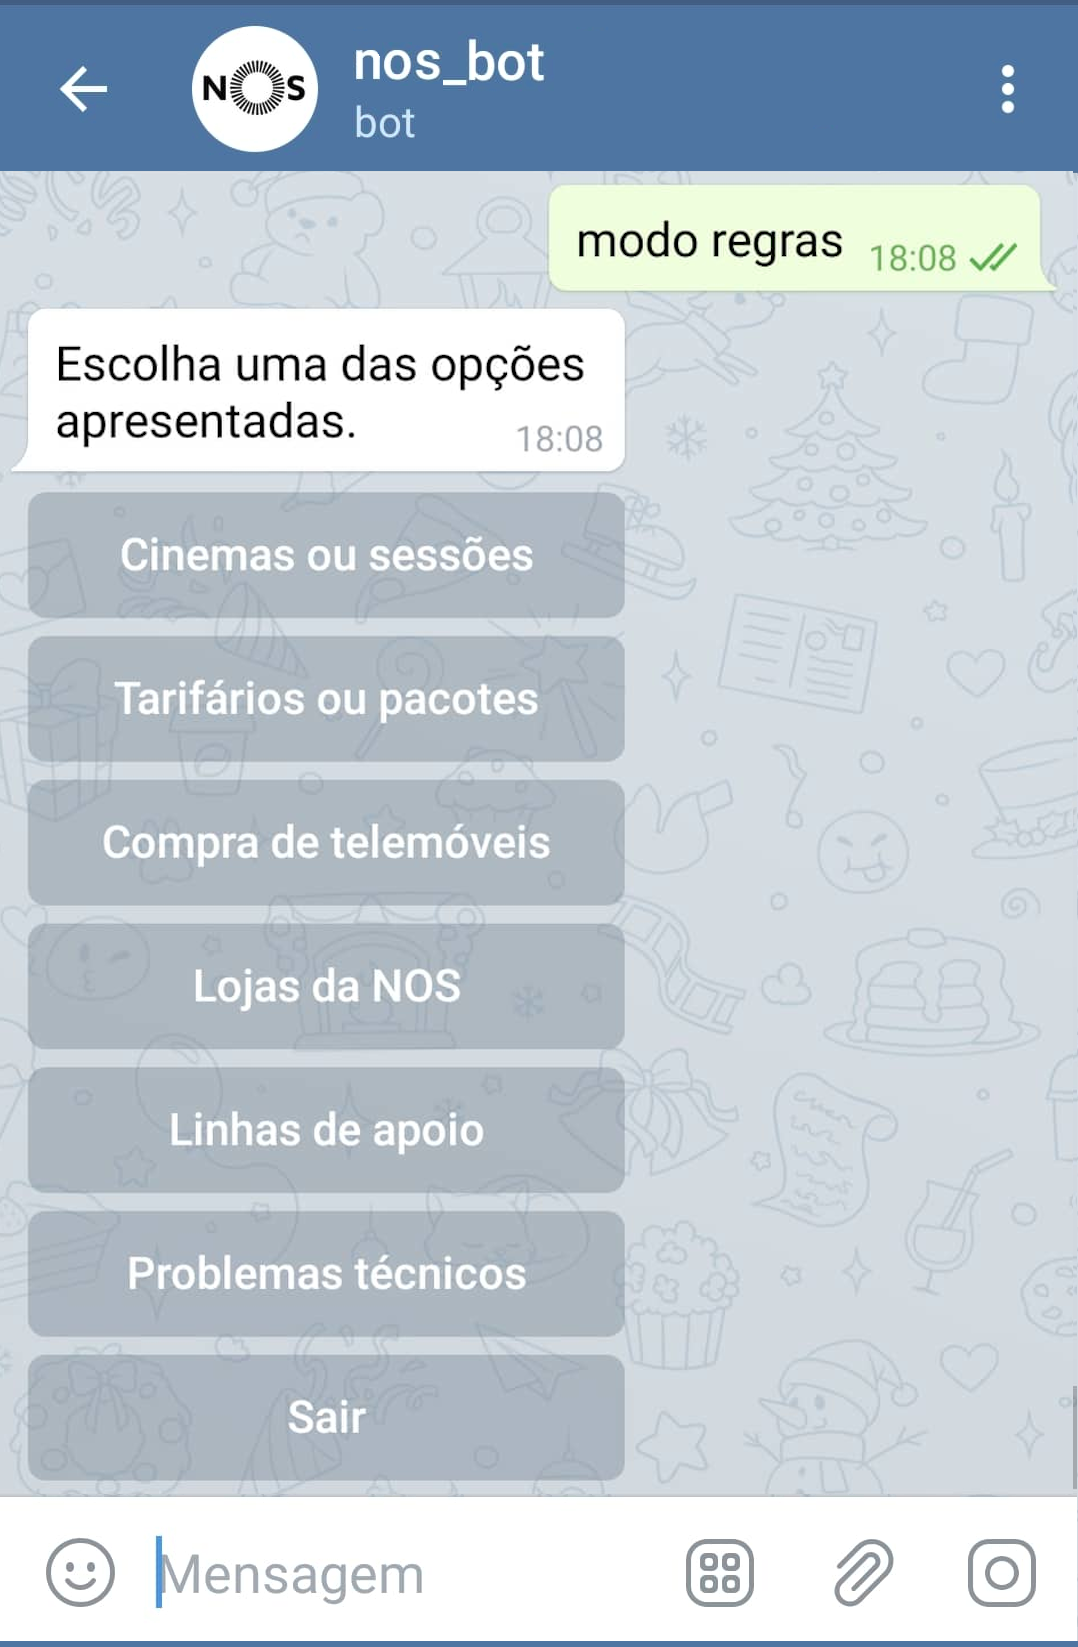
\includegraphics[width=0.30\textwidth]{images/modo_regras.png}
\end{center}
\caption{Menu principal do Modo de Regras}
\label{fig:figModoRegras}
\end{figure}

Para além de facilitar a experiência do utilizador, uma das principais vantagens deste modo está no processo
de pesquisa. Ao apresentar todas as opções ao utilizador de uma vez, este pode especificar o que pretende
filtrar na sua pesquisa e pedir para serem apresentados os resultados quando não pretender aplicar mais
filtros.


\subsection{Cinemas Webscraper}\label{sec:cinemas}

Este serviço tem como objetivo obter, e disponibilizar, as informações relacionadas com os cinemas NOS,
nomeadamente sobre os seus cinemas, filmes e as respetivas sessões, de forma a poder expor uma API
através da qual o \textit{Chat Processor} consiga obter informações que vão de encontro ao pretendido pelos
utilizadores do \textit{bot}.

\vspace{2mm}

Não tendo nós qualquer acesso a uma base de dados interna da própria NOS, o processo de obtenção da informação
necessária passa por fazer \emph{scraping} às páginas do \emph{website} da NOS que detêm informações sobre os
seus cinemas (\url{http://cinemas.nos.pt/}).

\vspace{2mm}

Numa fase inicial de estudo do desenvolvimento deste serviço, a primeira decisão passou pela escolha das
tecnologias a utilizar. Sendo assim, tendo em conta a familiaridade com \texttt{Python} por parte dos
membros do grupo encarregues do desenvolvimento deste componente, a juntar a uma maior facilidade e
experiência passada em realizar \emph{scraping} com esta linguagem, foi tomada a decisão que \texttt{Python}
seria a linguagem a utilizar. De seguida, tendo em conta que o objetivo passava por construir uma API REST e
também que seria útil ter uma ligação a uma base de dados para guardar os dados obtidos a partir da recolha
de informações do site, foi considerada que a utilização da \emph{framework} Django era uma escolha correta,
visto que simplificaria o processo de criação de \emph{endpoints} para a API, e permitiria utilizar uma base
de dados SQLite para armazenar e ler todas as informações necessárias, incluindo um ORM.

\vspace{2mm}

Relativamente ao comportamento do serviço, este pode ser dividido em duas partes/fases: obtenção de dados 
e a posterior disponibilização dos mesmos.

O processo de obtenção de dados, é feito como referido anteriormente, através de \emph{scraping}. Esta
recolha de dados é feita com recurso a diversas bibliotecas \texttt{Python}, nomeadamente a biblioteca
\texttt{requests} para conseguir obter o HTML das páginas, o \texttt{BeautifulSoup} que permite fazer um
\emph{parsing} mais facilitado das mesmas e obter certas \emph{tags} mais rapidamente, assim como a
biblioteca \texttt{re} que permite a utilização de expressões regulares para filtrar dados de
acordo com o pretendido. Os dados recolhidos são então guardados na base de dados \texttt{SQLite}, cujo
modelo é apresentado na figura abaixo.

\begin{figure}[H]
  \centering
  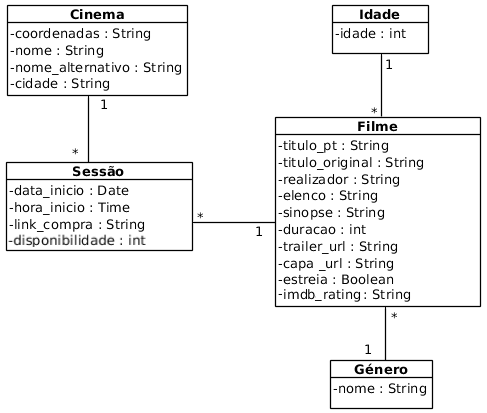
\includegraphics[width=8cm]{images/Cinemas_NOS_DB.png}
  \caption{Diagrama ER da base de dados do \textit{Cinemas Webscraper}.}
  \label{fig:cinemas_er_diagram}
\end{figure}

Desta forma, cada cinema NOS tem o seu conjunto de sessões, com indicação da data e da hora de início das
mesmas, assim como um \emph{link} através do qual o utilizador poderá comprar um bilhete para uma sessão, e
ainda a disponibilidade, que indica o número de lugares disponíveis, que mais à frente é referido
novamente. Neste modelo, uma sessão corresponde à exibição de um determinado filme que, para de entre as
várias informações sobre o mesmo, é armazena as entidades \texttt{Idade} e \texttt{Género}, de forma a
facilitar a filtragem de filmes tendo em conta o género procurado pelo utilizadores, ou até por restrições
de idade que possam estar associadas à pesquisa de filmes, por exemplo, para permitir aos utilizadores
procurar filmes com os quais possam assistir juntamente com os seus filhos.

\vspace{2mm}

A atualização destes dados é conseguida através da execução, periódica, do processo de \textit{scraping} já
referido. Para tal foram utilizadas \emph{tasks} \texttt{Celery} juntamente com a \emph{framework}
\texttt{Django}. A operação de recolha de filmes em exibição (ou das próximas estreias) e informações sobre
todas as sessões é feita todas as quintas-feiras entre as 5 e as 6 horas da manhã. Esta escolha deve-se ao
facto de o dia de quinta-feira ser quando as informações sobre os cinemas no site da NOS são atualizadas. No
entanto, tendo em conta que esta atualização só seria feita de uma em uma semana, a indicação dos lugares
livres numa sessão deixaria de fazer sentido, pois estaria praticamente sempre errada comparativamente ao
momento de apresentação dessa informação. Assim, esta atualização ,dos lugares livres de todas as sessões, é
realizada de uma em uma hora, de forma a impedir que a informação se torne obsoleta e impedir uma degradação
no desempenho do sistema, em consequência deste processo. Ainda assim, o desafio desta parte não se fica por
aqui, pois supondo que na base de dados num dado momento existem 7000 sessões (número realista tendo em
conta os testes realizados), isto significa que para atualizar a informação sobre estas sessões seria
necessário consultar 7000 páginas diferentes, introduzindo um \textit{overhead} considerável. Numa fase
inicial esta tarefa foi implementada de uma forma sequencial, mas supondo que cada pedido com a biblioteca
\texttt{requests} demore 1 segundo, levaria praticamente 2 horas a conseguir executar esta tarefa. Sendo
assim, a solução passou por utilizar várias \emph{threads} para realizar esta tarefa. Utilizando a
biblioteca \texttt{multiprocessing}, utilizam-se assim 15 diferentes processos para reduzir
consideravelmente o tempo de execução desta tarefa.
\vspace{2mm}

Importante ainda realçar que o atributo \texttt{imdb\_rating} da tabela \texttt{Filme}, apresentado na
Figura \ref{fig:cinemas_er_diagram}, foi implementado em resultado do \textit{feedback} resultante da
primeira fase de testes de usabilidade ao \textit{bot}. Na opinião de algumas pessoas seria relevante nas
informações sobre um filme apresentar também qual o \emph{rating} do mesmo no site
\href{https://www.imdb.com/}{IMDb}, como uma forma de verificar a qualidade ou não de um filme. Tendo em
conta que as páginas NOS não têm qualquer informação deste tipo, foi então necessário utilizar uma API
externa para poder obter estes dados. A escolha recaiu pela utilização da
\href{http://www.omdbapi.com/}{OMDb API}, para a qual a obtenção de um \emph{token} que permite obter acesso
às informações da mesma é fácil e gratuito. Desta forma, no momento em que se realiza a operação semanal de
recolha de informações sobre todos os filmes, é feito um pedido a esta API para cada filme, indicando para
além do \emph{token}, o nome do filme a pesquisar e o seu ano, informações que temos do nosso lado, por
exemplo:

\small{
\begin{verbatim}
http://www.omdbapi.com/?apikey=<API_TOKEN>&t=Jumanji&y=2019
\end{verbatim}}

A obtenção da informação resultante dos dados anteriormente referidos, por parte do \textit{Chat Processor},
é feita através dos \emph{endpoints} que este serviço expõe, que devolvem respostas no formato JSON
e, de forma sucinta, permitem realizar as seguintes ações:

\begin{enumerate}
    \item Procurar cinemas ou obter os cinemas mais próximos.
    \item Procurar os filmes em exibição num cinema.
    \item Procurar filmes com filtros como género, elenco, realizador, sinopse ou restrições de idade.
    \item Procurar as próximas estreias dos cinemas NOS.
    \item Obter detalhes de um filme.
    \item Procurar as próximas sessões.
    \item Procurar sessões de um filme em específico.
    \item Procurar sessões de filmes abaixo de uma determinada duração.
    \item Procurar sessões por data.
\end{enumerate}

Uma nota importante relativamente a estes \emph{endpoints}, excluindo os métodos 3, 4 e 5 apresentados em
cima, diz respeito à necessidade de receber, como parâmetros, ou as coordenadas (latitude-\texttt{lat} e
longitude-\texttt{lon}) do utilizador ou um termo de pesquisa (\texttt{search\_term}) que corresponda a uma
localização ou centro comercial, necessários à obtenção de informações como sessões em cinemas perto do
utilizador ou de acordo com a localização pretendida pelo mesmo.

A título de exemplo, no método que permite a procura de cinemas, inicialmente, se fossem passados os valores
de latitude e longitude eram devolvidos os cinemas que se encontram a uma distância máxima de 20 Km
(calculada com a Fórmula de Haversine) e, se fosse em alternativa passado um termo de pesquisa eram apenas
devolvidos os cinemas que fizessem \emph{match} com essa mesma procura. No entanto, com a realização de
algumas validações e utilização por parte de pessoas externas à equipa de desenvolvimento, esta abordagem
foi alterada no sentido de melhorar o fornecimento de informações ao utilizador. Desta forma, quando são
passados os valores de latitude e longitude, e nos casos em que não existam cinemas num raio de 20 Km, é
devolvido o cinema mais próximo das coordenadas indicadas. No caso em que é passado um termo de pesquisa,
imaginemos, o nome de um Concelho português, no caso de não fazer \emph{match} com nenhum cinema, obtemos as
coordenadas (latitude e longitude) dessa localização, utilizando a biblioteca \texttt{geopy}, e é feita a
procura de quais os cinemas que se encontram num raio de 20 Km tendo em conta essa mesma localização, ou o
mais perto no caso de não existir nenhum nessa mesma ``circunferência''.

\subsection{FS Webscraper}\label{sec:fs_scrapper}
Esta componente tem como objetivo disponibilizar informações relacionadas com serviços que são
providenciados no site da NOS, nomeadamente os telemóveis à venda, pacotes de televisão e linhas de apoio, e
no site da WTF, nomeadamente os tarifários existentes. Para tal, utilizou-se a \textit{framework}
\textit{Flask} para facultar uma API através da qual o \textit{Chat Processor} consegue obter as informações
necessárias de acordo com o pedido dos utilizadores do Bot.

Relativamente aos \emph{endpoints} expostos na API deste serviço, nestes são devolvidas as informações num
formato JSON e, de forma sucinta, existem métodos que permitem realizar as seguintes ações:

\begin{enumerate}
    \item Consultar linhas de apoio.
    \item Procurar telemóveis por marca, novidades, em desconto, mais pesquisados, que vêm com uma oferta,
    que podem ser pagos por prestações ou com pontos e/ou num intervalo de preço.
    \item Consultar tarifários WTF disponíveis.
    \item Procurar por lojas disponíveis numa região ou perto de coordenadas fornecidas.
    \item Procurar pacotes com base no nome, tipo, serviço e/ou intervalo de preço.
\end{enumerate}

As informações obtidas relativas às ações descritas acima são recolhidas via \textit{scraping} aos sites da
NOS e WTF. Dada a diversidade de serviços disponibilizados e a inexistência de relações entre os mesmos,
concluiu-se que não faria sentido utilizar uma base de dados relacional. Foi ponderada a utilização de uma
base de dados não relacional em Mongo DB, no entanto, para utilizar a mesma iria ser necessário ter mais uma
componente em execução. O facto do conteúdo retirado possuir uma dimensão reduzida levou a que se
armazenasse os dados em ficheiros JSON, devidamente estruturados, não comprometendo a escalabilidade do
projeto. Esta opção foi decisiva para a escolha do \textit{Flask}, pois não seria necessário uma
\textit{framework} pesada para gerir uma base de dados. Os ficheiros gerados são os seguintes:

\begin{itemize}
    \item \textbf{linhas\_apoio.json} - Contém informações relativas às linhas de apoio da NOS. Este
      ficheiro é de elevada importância na medida em que, quando no modo de resolução de problemas não é possível
      ajudar o utilizador, é fornecido ao mesmo o contacto de uma linha de apoio que lhe possa ser útil.
    \item \textbf{lojas.json} - Contém todas as informações relativa às lojas da NOS como a sua localização, horário
      de funcionamento e lista de serviços disponíveis na mesma.
    \item \textbf{pacotes.json} - Contém informações relativas aos pacotes de fibra e satélite presentes no
      site da NOS, incluindo todas as opções de fidelização e respetivo custo.
    \item \textbf{phones.json} - Contém informações relativas aos telemóveis para venda presentes no site da NOS.
    \item \textbf{top\_phones.json} - Contém informações dos telemóveis mais vendidos pela NOS. 
    \item \textbf{tarifario\_WTF.json} - Contém informações relativas aos tarifarios WTF da NOS.    
\end{itemize}

Tal como no caso dos cinemas, é disponibilizado ao utilizador a possibilidade de averiguar quais as lojas
mais próximas da sua localização. O cálculo é efetuado através da Fórmula de Haversine. Ao contrário dos
cinemas, dado o elevado número de lojas da NOS, especialmente nos grandes centros urbanos, são apenas
apresentadas as 4 lojas mais próximas do utilizador.

Relativamente a atualizações dos ficheiros JSON, estas são realizadas com frequências diferentes. No caso
das lojas, é realizado um \textit{update} a cada 168 horas. Relativamente aos outros serviços, a atualização
é feita a cada 24 horas, visto que os mesmos contêm informações que se alteram com mais frequência.


\subsection{Resoluções técnicas}\label{sec:resTec}
O módulo de resolução de problemas técnicos representa uma das partes integrais do sistema desenvolvido,
visto que permite aos clientes da NOS agilizar o processo de \textit{troubleshooting} ao permitir que
iniciem o mesmo sem ser necessário contactar um operador "humano". Dada a complexidade deste componente,
que combina processamento de linguagem natural na extração de tipificações com \textit{machine learning}
para o cálculo das soluções, o serviço foi dividido em duas componentes distintas:

\begin{itemize}
    \item \textbf{NTP Bot}: responsável por mapear o \textit{input} do utilizador em tipificações (internas)
    usadas pelo sistema
    \item \textbf{NTP Solver}: responsável por sugerir um conjunto de soluções, tendo em conta os dados relativos
    ao cliente
\end{itemize}

Neste serviço a interação com o exterior é feita através do NTP Bot, cuja API expõe um único
\textit{endpoint} através do qual é feita toda a interação a partir do momento em que o \textit{Chat Processor}
deteta que o utilizador pretende interagir com este módulo.

\subsubsection{Fluxo de Execução}
Dada as particularidades deste módulo, é importante perceber como se processa o fluxo de execução normal
que, tal como nos restantes módulos, se inicia no momento em que o \textit{Chat Processor} identifica o intuito do
utilizador. A partir desse momento o \textit{Chat Processor} passa a servir de \textit{proxy} às mensagens do
utilizador até receber indicação do NTP Bot (ou através da mensagem \texttt{/reset}) que a interação com o
módulo terminou, limitando-se a converter as mensagens para a estrutura JSON esperada pelo
mesmo. Previamente a qualquer interação com o \textbf{NTP Solver}, o utilizador é obrigado a autenticar-se
como cliente da NOS, utilizando como fatores de autenticação o número de telemóvel e o NIF associados ao seu
contrato. Quando a autenticação é realizada com sucesso, é estabelecida uma sessão HTTP entre o NTP Bot e
NTP Solver, necessária para fazer pedidos aos endpoints expostos pelo primeiro. A gestão destas sessões é
feita automaticamente pela \textit{framework} Django usada pelo NTP Solver, que também armazena os dados
relativos ao contrato de cada cliente:

\begin{figure}[H]
    \centering
    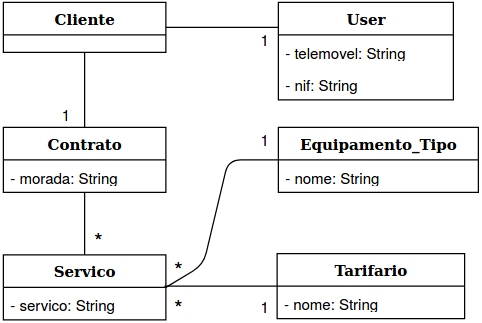
\includegraphics[width=7cm]{images/NTP_Solver_DB.png}
    \caption{Diagrama ER da base de dados do NTP Solver}
    \label{fig:ntp_er_diagram}
\end{figure}

Estes dados, em conjunto com as tipificações extraídas a partir das descrições do problema providenciadas
pelo cliente, servem de \textit{input} ao modelo que é responsável por encontrar uma solução para o problema
em causa. O resultado deste modelo consiste num conjunto de (no máximo) três soluções distintas que são
apresentadas ao cliente de maneira iterativa \textbf{i.e.} quando o cliente indica que a solução anterior
não resolveu o seu problema. Em último recurso o módulo indica as linhas de apoio da NOS referentes ao
serviço no qual o cliente está a experienciar o problema. Visto ser um serviço com uma dependência
considerável em \textit{machine learning}, o mesmo foi desenvolvido com o intuito de ser capaz de melhorar,
ao longo do tempo, a sua capacidade de resolver problemas. Para isso, cada vez que um utilizador interage
com o sistema e indica que o seu problema foi resolvido com sucesso, os dados de entrada e saída do modelo
referentes a esse problema são armazenados num ficheiro CSV, sendo posteriormente usados para voltar a treinar o modelo.
\newline

\textbf{NTP Bot}

Dado o seu papel na interação com utilizador e extração de dados para a resolução de problemas, o NTP Bot é
um dos componentes fundamentais do módulo NTP, sendo útil perceber como este funciona. Uma das suas funções,
a extração de problemas, tem como intuito mapear descrições, de natureza coloquial, provenientes dos
clientes em tipificações usadas pelo modelo. Para isso, o processo de mapeamento encontra-se dividido em
duas fases distintas, uma primeira que realiza a substituição de termos presentes no \textit{input} do
cliente em termos usados nas tipificações (\textbf{e.g} fibra $\mapsto$ FTTH) por forma a aproximar este
discurso da terminologia usada pelas mesmas. Uma segunda fase que mapeia todas as versões resultantes destas
substituições nas tipificações das quais estas mais se aproximam em termos semânticos, recorrendo para isso
a técnicas de cálculo de semelhança semântica (utilizando o modelo de TensorFlow
\texttt{universal-sentence-encoder-multilingual-large}). Este processo, apesar de apresentar resultados
aceitáveis, representa um \textit{bottleneck} na capacidade de resposta do sistema, visto que os modelos
existentes de processamento de linguagem natural portuguesa estão preparados para um discurso informal,
contrário ao usado para as tipificações. Assim sendo, este mapeamento apenas é aceite quando a confiança no
mesmo é superior a um determinado valor, sendo necessário pedir ao utilizador uma descrição mais detalhada
quando isto não se verifique.
\newline

\textbf{NTP Solver}

A resolução de problemas e autenticação dos clientes é realizada pelo componente NTP Solver que, tal como o
serviço \textit{Cinemas Webscraper}, recorre à \textit{framework} Django para implementar uma API REST com ligação à
base de dados que armazena os dados dos contratos de cada cliente NOS. Quando um cliente inicia a interação
com o módulo e indica o serviço no qual está a experienciar problemas, dados como o equipamento e tarifário
são usados em conjunto com as tipificações mapeadas pelo NTP Bot para obter uma solução para a situação
particular do cliente. Nesse sentido, este sub-módulo disponibiliza os seguintes \textit{endpoints}:
\begin{itemize}
    \item \texttt{/login}
    \item \texttt{/logout}
    \item \texttt{/client\_has\_service}           
    \item \texttt{/solve}
    \item \texttt{/update\_log}
\end{itemize}

sendo os dois primeiros responsáveis pela gestão das sessões HTTP requeridas pelos dois últimos. A interação
com o modelo de resolução de problemas é realizada através do penúltimo \textit{endpoint}, que recebe as
tipificações do problema como parâmetros GET e devolve uma lista de possíveis soluções (no máximo 3), cuja
confiança seja superior a 70\%. Dadas tipificações devolvidas pelo modelo serem de teor técnico,
dificultando a interpretação das mesmas por clientes com pouco conhecimento tecnológico, este módulo mapeia
ainda as mesmas em expressões ``informais''. O último \textit{endpoint} permite que o modelo seja treinado
de maneira automática, periodicamente. Para isso, este recebe um ficheiro CSV em que cada entrada
representa uma resolução de problemas realizada com sucesso, incluindo os dados de entrada do modelo e o
\textit{output} que permitiu solucionar o problema descrito. Quando o número de entradas novas atinge 15000,
o modelo volta a ser treinado, tendo este valor sido escolhido com base na relação entre a precisão do modelo e o
número de amostras usadas no seu treino:

\begin{figure}[H]
    \centering
    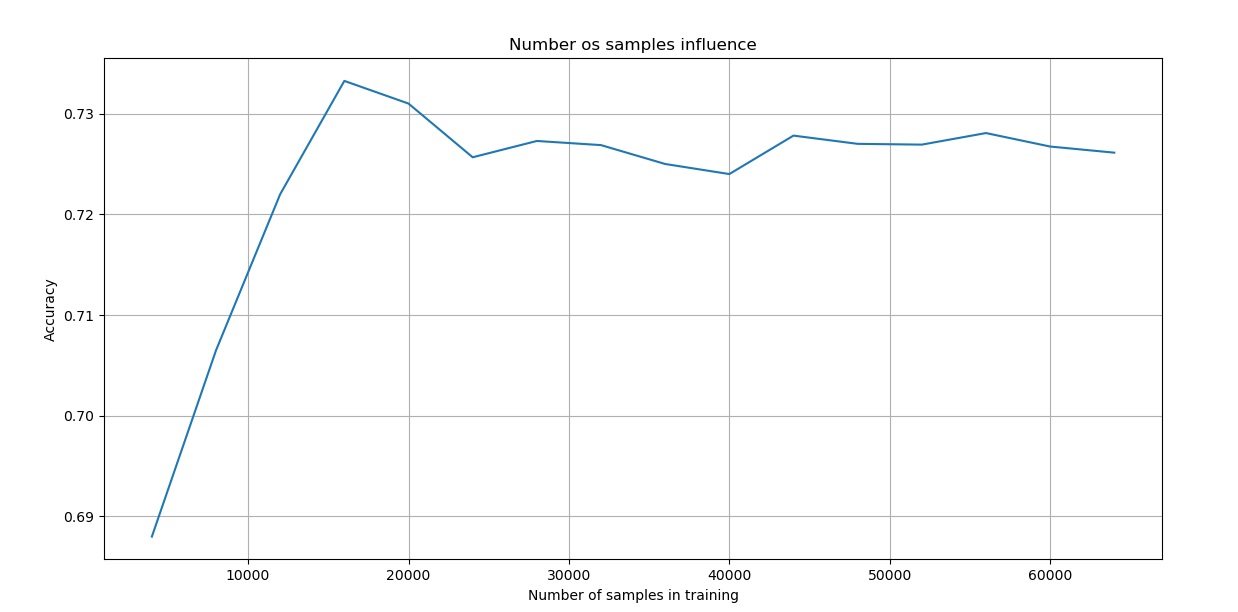
\includegraphics[width=13cm]{images/n_samples_influence.png}
    \caption{Tamanho da amostra vs. Confiança}
    \label{fig:sample_size_accuracy}
\end{figure}

\subsubsection{Modelo de classificação}

O componente NTP Solver utiliza um modelo de classificação criado com base nos dados fornecidos pela NOS.
Para a construção deste modelo foram utilizadas várias ferramentas de \textit{python} como \textit{numpy} e
\textit{pandas} para o tratamento dos dados , além do \textit{sklearn} e \textit{keras} para a utilização
dos algoritmos de classificação de \textit{machine learning}.  O processo de implementação do modelo segue
as seguintes fases:
\begin{itemize}
    \item Visualização e pré-processamento dos dados
    \begin{itemize}
        \item Visualização dos dados
        \item Identificação e tratamento do \textit{target}
        \item Tratamento dos dados em falta ou nulos
        \item Adaptação das linhas com \textit{target's} menos frequentes
        \item Discretização dos dados
        \item \textit{Feature Selection}
        \item Divisão balanceada dos dados(75\% de treino e 25\% de teste)
    \end{itemize}
    \item Treino e teste dos modelos  com \textit{Hyper parameter optimization} (\textit{Grid Search})
    \begin{itemize}
        \item Árvore de Decisão
        \item \textit{Support Vector Machine}
        \item \textit{K-nearest neighbors}
        \item \textit{Naive bayes}
        \item \textit{Random Forest}
        \item \textit{Logistic regression}
        \item Rede neuronal artificial
    \end{itemize}
    \item Avaliação dos modelos
\end{itemize}
O modelo final consegue responder com 30 classes/resoluções distintas, através das seguintes \textit{features} :
\begin{itemize}
    \item Serviço -  Internet, Voz ou TV
    \item Tarifário -  Tarifário do cliente
    \item Equipamento -  Equipamento com o problema
    \item Sintoma -  Sintoma do problema reportado pelo cliente, traduzido pelo assistente
    \item Tipificações Nível 1, 2 e 3 - Tipificações atribuídas pelo assistente no momento do atendimento
\end{itemize}

\section{Deployment}
O processo de \textit{deployment} é de extrema importância, visto que permite garantir que os componentes
desenvolvidos estão funcionais e que conseguem comunicar entre si.  Dada a modularidade do projeto, que se
encontra divido em microserviços, para o deployment recorreu-se ao uso do \textit{Docker}. Nesse sentido,
para cada componente foi criada uma imagem \textit{Docker} com todas as dependências necessárias à sua
execução. Com recurso ao \texttt{docker-compose}, que permite a execução e gestão (orquestração) de vários
\textit{containers} (execução de uma imagem), é obtido o \textit{deployment} do projeto.

\section{Resultados e Conclusões}
Em termos de reconhecimento de entidades e categorização da funcionalidade pretendida pelo utilizador na
linguagem natural, o \textit{Chat Processor} carece de melhorias, apesar de que estas são um trabalho
progressivo entre testes de usabilidade com utilizadores por forma a assimilar a escrita das questões pelos
mesmos e a adição do reconhecimento dessas expressões. Relativamente ao modo regras, este teve uma boa
receção por parte dos utilizadores e por parte da empresa, devido aos botões utilizados, que o tornaram mais
intuitivo e direto. Estes botões permitiram-nos tirar partido das funcionalidades do \textit{Telegram}. No
entanto, no caso de se pretender alterar o serviço de mensagens utilizado, o modo de regras foi desenvolvido
de maneira a que esta transição seja simples, não sendo um obstáculo.

Um problema transversal aos micro-serviços que obtêm dados de fontes como \textit{websites}, através de
técnicas de \textit{scraping}, prende-se com a volatilidade inerente a fontes deste tipo. Esta
característica leva a que, modificações no código fonte das páginas, possa impedir que a informação seja
corretamente obtida sem que haja modificações no código que realiza o \textit{scraping}, ainda que o sistema
tenha sido desenvolvido para tolerar estas modificações sem comprometer o seu funcionamento. Para além
disso, um obstáculo neste trabalho apresentou-se no facto de o desenvolvimento destes \textit{scrapers} ter
consumido uma porção de tempo significativa, devido à complexidade dos sites. Numa futura implementação
deste projeto (ou continuação), ao invés de obter a informação a partir de \textit{web scrapers}, o acesso a
uma base de dados com a informação pretendida facilitaria a recolha dos mesmos, bem como tornaria o processo
mais viável, pois deixaria de existir o risco de se perder o acesso à informação com a alteração dos
\textit{websites}.

De forma semelhante ao que se verifica no \textit{Chat Processor}, o reconhecimento de linguagem natural no
\textit{NTP Bot}, sub-módulo do componente de resolução de problemas, representa o maior \textit{bottleneck}
no que diz respeito à capacidade de resolução de problemas. A disparidade entre os termos utilizados pelos
utilizadores, de natureza coloquial, e os utilizados para descrever as tipificações de problemas leva a que
técnicas de semelhança semântica não apresentem o desempenho desejado, apesar do uso das mesmas em conjunção
com dicionários de sinónimos para mapeamento de termos informais em técnicos. Por outro lado, e no sentido
oposto, as soluções apresentadas pelo sistema verificam o mesmo problema, encontrando-se num formato de alto
teor técnico que dificulta a sua compreensão por parte dos utilizadores.

Apesar das suas limitações, em parte provocadas pela escassez de modelos de processamento de linguagem natural
com suporte para língua portuguesa, a realização de testes de usabilidade e os resultados obtidos permitem
concluir que o sistema desenvolvido facilita o acesso a serviços da NOS ao promover a centralização dos mesmos
num \textit{hub} comum. 
Recorrendo aos requisitos definidos no início do processo de desenvolvimento como referência \ref{anexo2}, é correto afirmar
que o projeto cumpre os objetivos principais estipulados. No entanto, como já foi mencionado anteriormente, 
este é um projeto onde existe sempre espaço para aperfeiçoamento e trabalho futuro, visto que a capacidade
de resposta do \textit{bot} dependem da sua interação com utilizadores.

\newpage

\begin{appendices}

\section{Modo de Regras - Máquinas de Estado}\label{anexo1}

\begin{figure}[H]
    \centering
    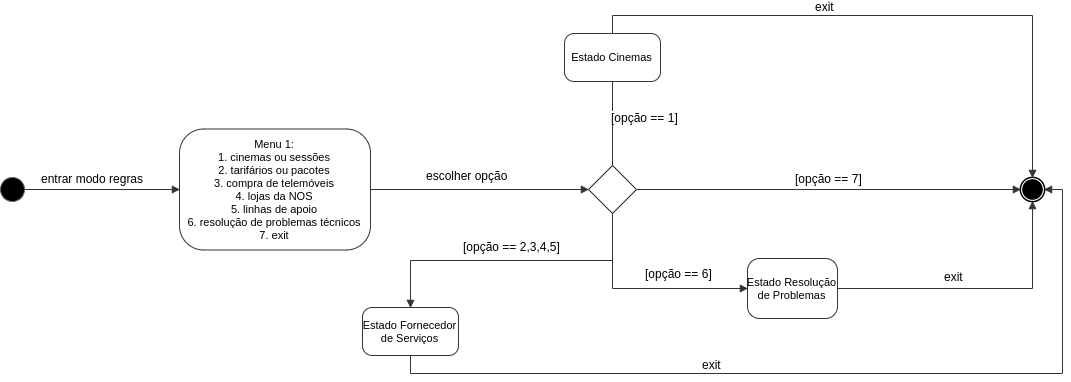
\includegraphics[width=15cm]{images/PEI_StateMachine-PEI_StateMachine.png}
    \caption{Diagrama de máquina de estados referente ao modo de regras - parte 1}
    \label{machine1}
\end{figure}

\begin{figure}[H]
    \centering
    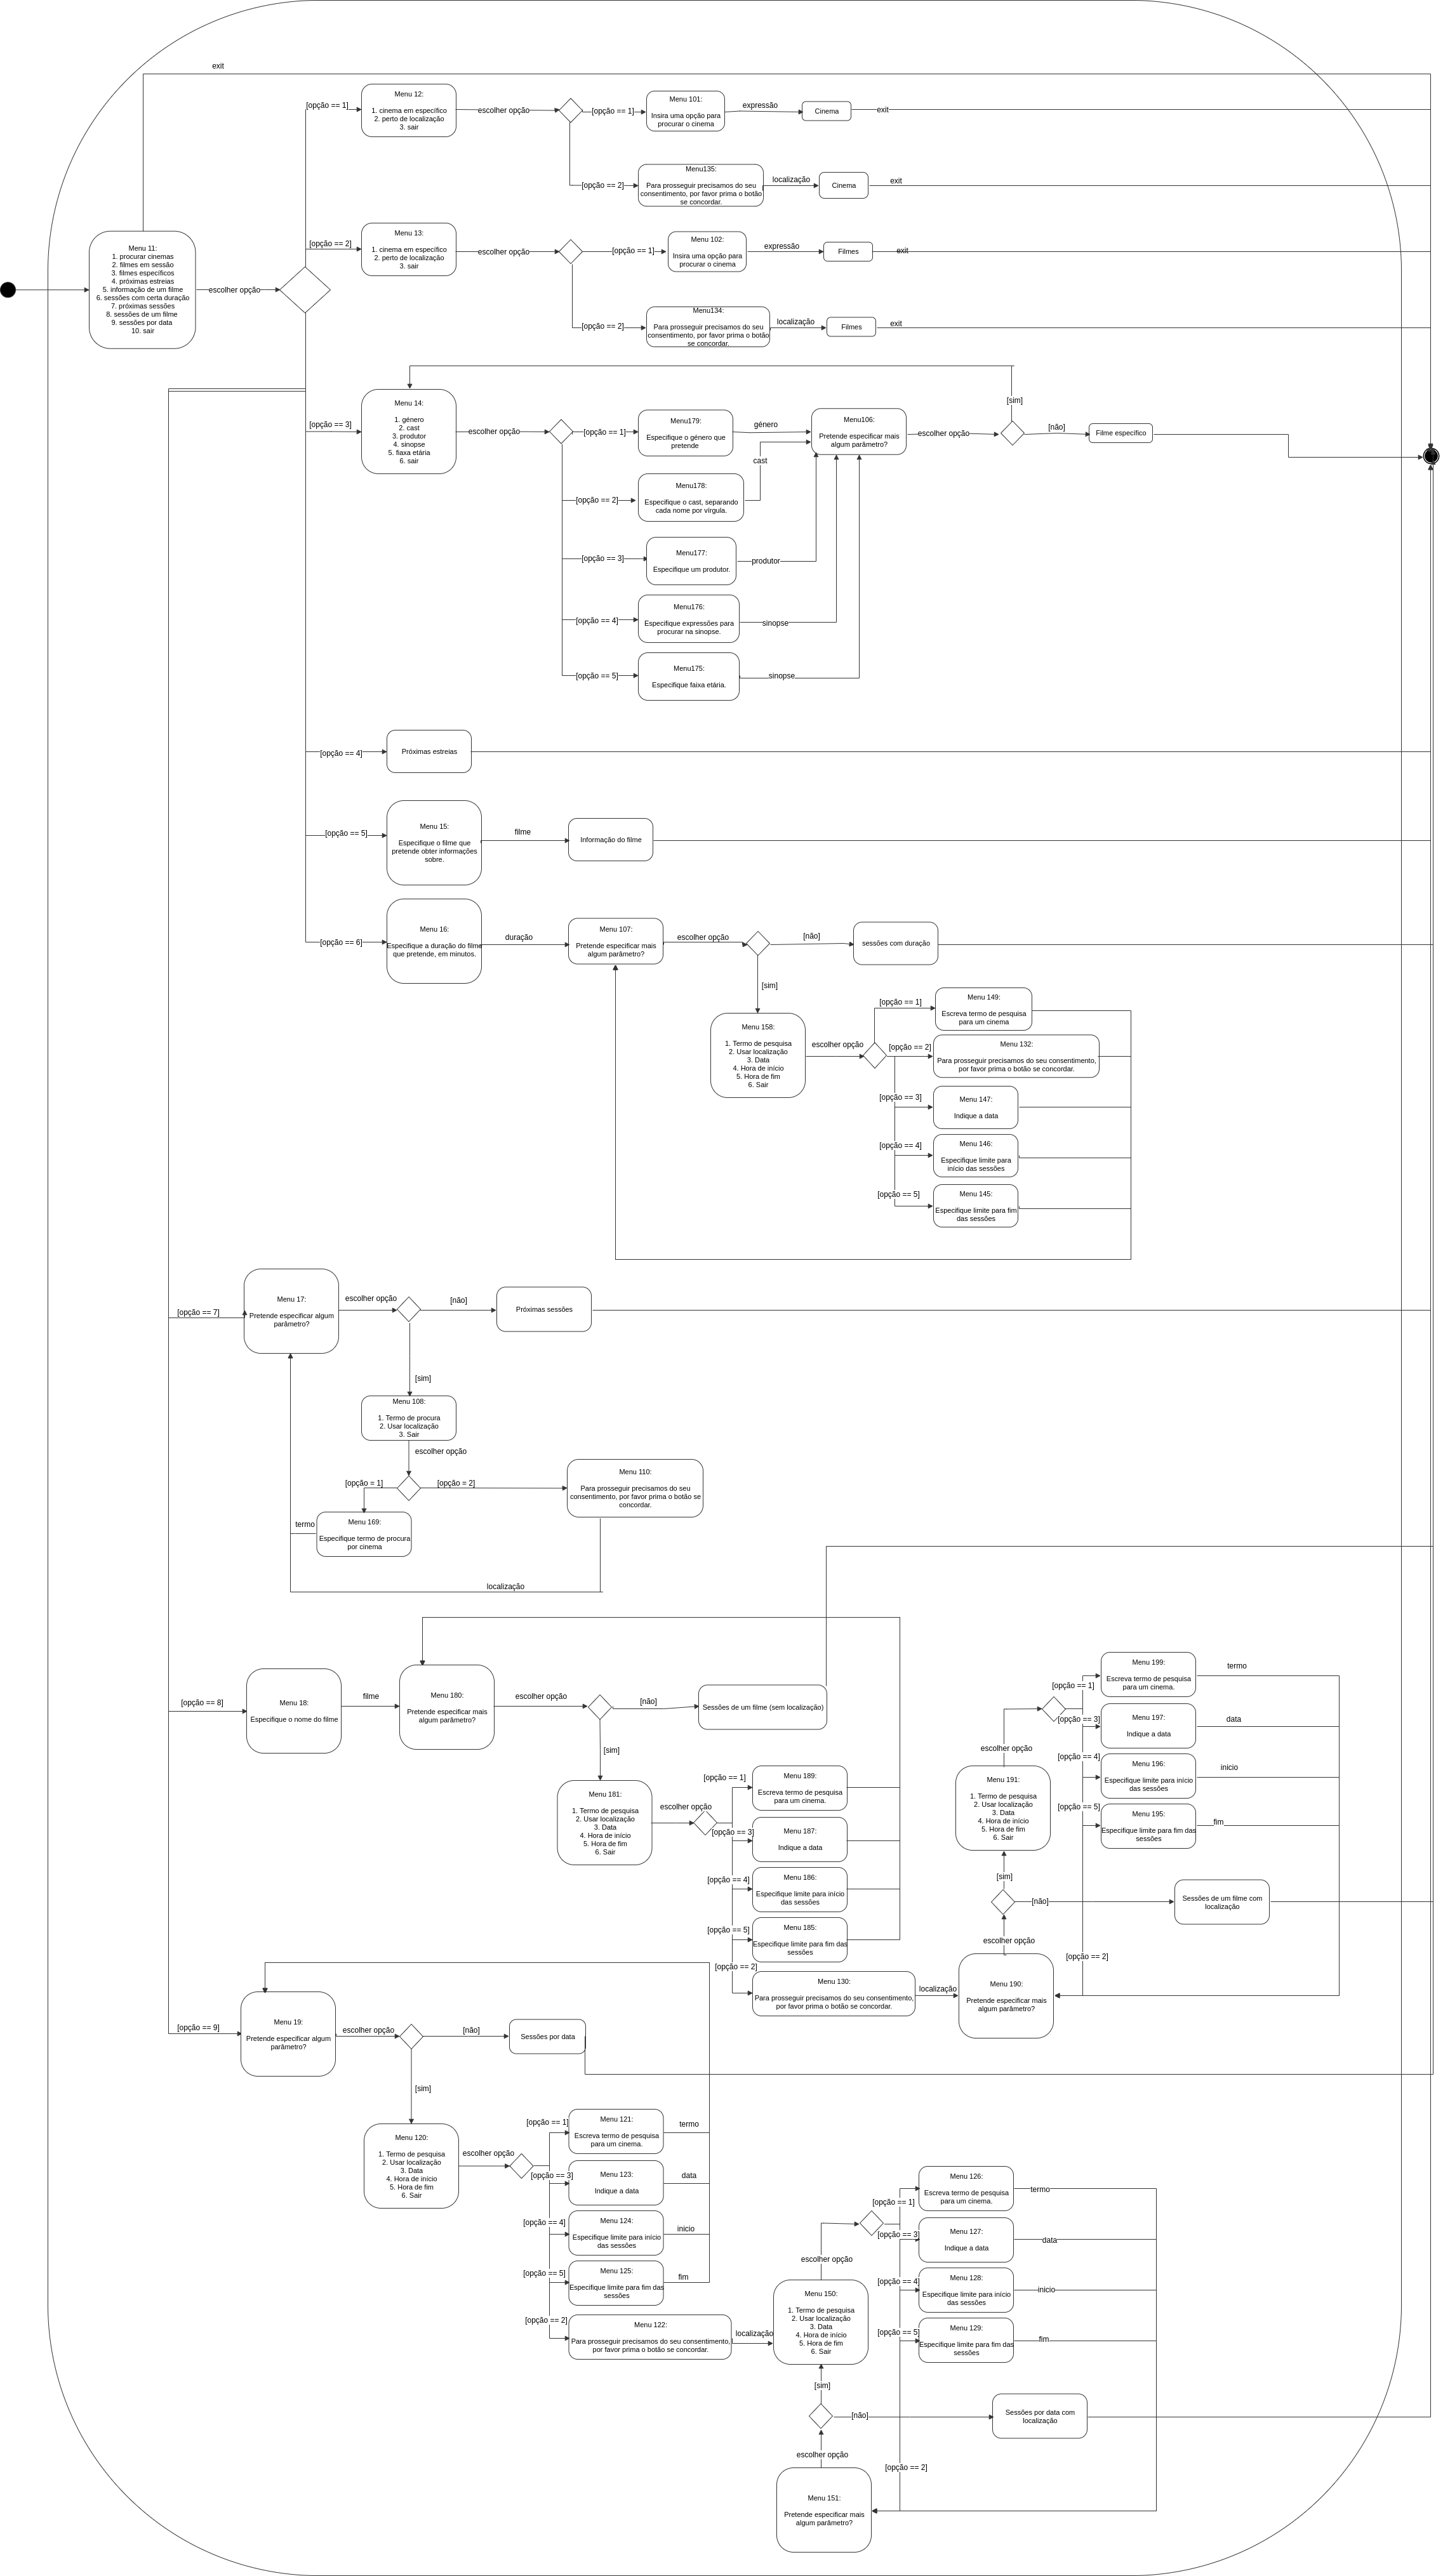
\includegraphics[width=12cm]{images/PEI_StateMachine-Cinemas.png}
    \caption{Diagrama de máquina de estados referente ao modo de regras - parte 2: Cinemas}
    \label{machine2}
\end{figure}

\begin{figure}[H]
    \centering
    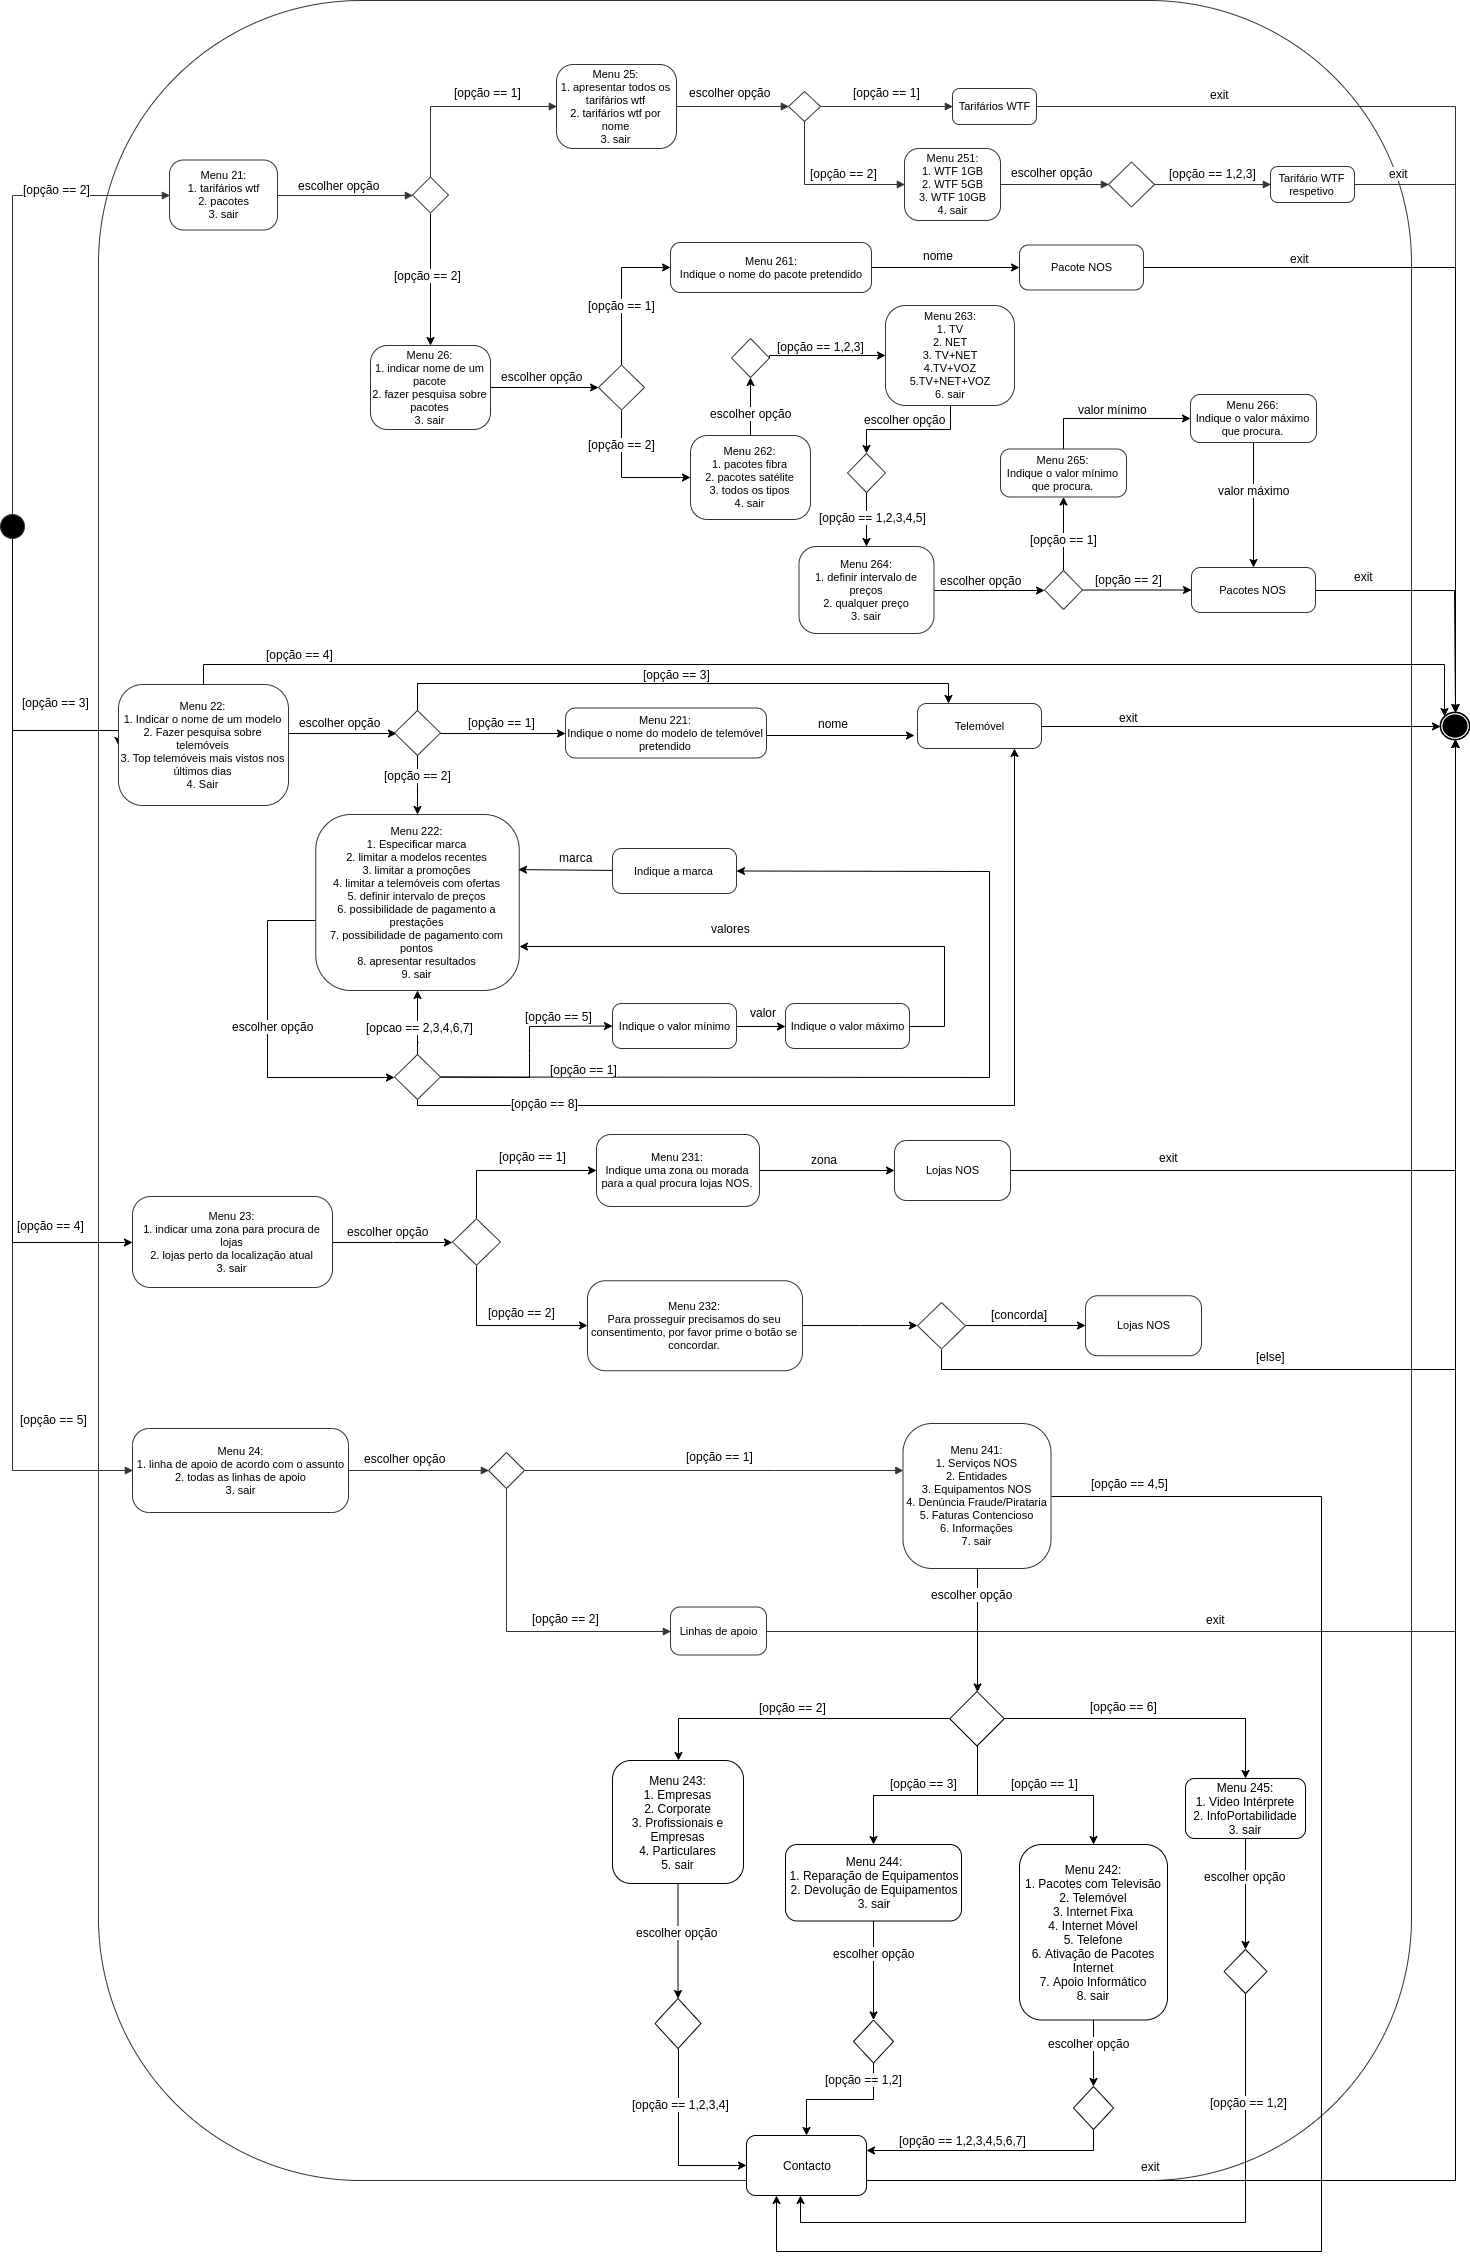
\includegraphics[width=12cm]{images/PEI_StateMachine-FornecedorServicos.png}
    \caption{Diagrama de máquina de estados referente ao modo de regras - parte 3: Serviços NOS}
    \label{machine3}
\end{figure}

\newpage

\section{Requisitos} \label{anexo2}

Os requisitos de seguida apresentados encontram-se no seguinte formato:
\begin{itemize}
    \item Descrição curta e concisa do requisito;
    \item Prioridade que o requisito terá na implementação do sistema.
\end{itemize}

A priorização dos requisitos foi obtida ao usar uma escala de classificação dos requisitos. Esta escala varia de 1 a 4 e permite dividir os requisitos em quatro grupos:
\begin{itemize}
    \item \textbf{1:} Requisitos que têm de ser satisfeitos pelo produto final;
    \item \textbf{2:} Requisitos que devem de ser satisfeitos pelo produto final;
    \item \textbf{3:} Requisitos que não são necessários para o produto final mas que lhe acrescem valor;
    \item \textbf{4:} Requisitos que podem eventualmente ser considerados na posterioridade.
\end{itemize}

\subsection{Requisitos Funcionais}
\subsubsection{Geral}
\begin{itemize}
    \setlength\itemsep{0em}
    \item \requirement{O sistema deve manter um estado para a conversa com cada cliente.}
    {É necessário determinar o contexto de uma mensagem enviada pelo utilizador.}{1}
    \item \requirement{O sistema deve disponibilizar dois modos de utilização: por discurso (interactivo) e por comandos}
    {A existência de dois modos de utilização facilita a adopção do sistema por parte dos clientes ao abranger
    um maior número de tipos de cliente.}{1}
    \item \requirement{O sistema deve ser capaz de lidar com variabilidade no \textit{input}.}
    {O sistema deve ser capaz de lidar com coloquialidade inerente ao discurso.}{1}
    \item \requirement{O sistema deve aceitar mensagens de áudio em alternativa a mensagens escritas.}
    {Facilidade de interação com o utilizador.}{4}
    \item \requirement{O sistema deve ser capaz de interpretar e categorizar a mensagem enviada pelo utilizador.}
    {O sistema necessita de perceber que componentes necessita de usar para responder ao utilizador.}{1}
    \item \requirement{Quando a categorização da mensagem é obtida com uma confiança superior de 65\% (inclusive)
    o sistema deve passar à obtenção de uma resposta para o utilizador.}
    {Garantir que se conhece a categoria do problema para poder responder conforme a necessidade do utilizador.}{1}
    \item \requirement{Quando a categorização da mensagem é obtida com uma confiança inferior a 65\% (exclusive) 
    o sistema deve pedir ao utilizador para reformular a pergunta.}
    {Garantir que se conhece a categoria do problema para poder responder conforme a necessidade do utilizador.}{1}
    \item \requirement{Ao fim de 5 tentativas abaixo de 65\% informa o utilizador das várias funcionalidades 
    disponibilizadas pelo sistema (modo por comandos).}
    {Quando o sistema não consegue perceber o que o utilizador pretende consultar, a melhor solução passa por entrar 
    num modo em que as várias possibilidades (comandos) de cada área disponível são apresentadas por passos ao utilizador.}{1}
    \item \requirement{Ao fim de 5 tentativas abaixo de 65\% informa o utilizador das várias linhas de apoio, 
    assim como os sites informativos ou lojas que possam satisfazer as suas necessidades.}
    {Quando o sistema não consegue perceber o que o utilizador pretende consultar, pode ser melhor indicar outros meios
    de obter as informações pretendidas.}{1}
    \item \requirement{O sistema deve ter um discurso fluido e variado.}{O sistema deve simular a interação com um assistente humano.}{2}
    \item \requirement
    {As listas apresentadas ao utilizador devem ser limitadas a 5 elementos.}
    {A apresentação de listas de 5 elementos permite evitar o sobrecarregamento de informação.}{2}
    \item \requirement{Quando o número de elementos for superior a 5, o utilizador deve
    poder visualizar mais elementos ao escrever "Ver mais".}
    {O utilizador deve ser capaz de visualizar todos os elementos que pretender.}{2}
\end{itemize}

\subsubsection{Resolução de problemas técnicos}
\begin{itemize}
    \setlength\itemsep{0em}
    \item \requirement{O cliente da NOS deve poder submeter um problema técnico e receber uma resposta de acordo com o mesmo.}
    {De forma a manter a satisfação e poder resolver os problemas dos clientes da NOS, a aplicação deve sempre enviar uma resposta 
    que considere ser a mais ajustada ao problema apresentado.}{1}
    \item \requirement{Uma resposta sugerida a um problema técnico com menos de 70\% de confiança não deve ser enviada.}
    {De forma a não induzir o cliente em erro, uma sugestão de resposta que não seja tomada como correta não deve ser enviada.}{1}
    \item \requirement{No caso da resposta sugerida a um problema técnico ter menos de 70\% de confiança deve ser recomendado ao cliente entrar em contacto com a área de apoio.}{O encaminhamento do cliente para a linha de apoio permite agilizar o atendimento do mesmo.}{1}
    \item \requirement{O sistema deve ser capaz de armazenar os dados relativos às resoluções técnicas dos utilizadores.}
    {Estes dados das resoluções obtidos a partir do nosso sistema podem ajudar a melhorar a precisão do nosso modelo de classificação.}{3}
    \item \requirement{O utilizador deve ser capaz de indicar se a solução sugerida resolveu o seu problema técnico.}
    {O \textit{feedback} dos utilizadores quanto à eficácia das soluções apresentadas é fulcral na melhoria do serviço.}{3}
    \item \requirement{O modelo de classificação de resoluções técnicas  do nosso sistema deve ser treinado com os novos dados recolhidos de 2 em 2 meses de forma automática.}
     {Certas classificações do nosso modelo podem deixar de ser as mais indicadas, por isso, para manter o modelo atualizado, automatizamos o treino do modelo com os eventuais dados recolhidos.}{3}
\end{itemize}

\subsubsection{Produtos e serviços disponibilizados pela NOS}
\begin{itemize}
    \setlength\itemsep{0em}
    \item \requirement{O utilizador deve poder consultar todos os números da linha de apoio.}
    {Quando o utilizador não tem a certeza do assunto mais adequado para a sua questão, deve-se 
    disponibilizar todos os números da linha de apoio de forma a facilitar a escolha por parte do utilizador.}{1}
    \item \requirement{O utilizador deve poder consultar o(s) número(s) da linha de apoio relativo a determinado assunto.}
    {A consulta do(s) número(s) da linha de apoio para determinado assunto permite aos utilizadores obter a ajuda adequada à sua questão.}{1}
    \item \requirement{O utilizador deve poder consultar um telemóvel tendo em conta o seu modelo.}
    {A consulta dos telemóveis por modelo permite aos utilizadores restringir a sua consulta ao item de interesse.}{1}
    \item \requirement{O utilizador deve poder consultar um telemóvel tendo em conta a sua marca.}
    {A consulta dos telemóveis por marca permite aos utilizadores restringir a sua consulta ao item de interesse.}{1}
    \item \requirement{O utilizador deve poder consultar o top de telemóveis mais vistos, disponíveis no site da NOS.}
    {A consulta do top de telemóveis mais vistos permite aos utilizadores obter informações sobre os telemóveis mais populares no momento.}{2}
    \item \requirement{O utilizador deve poder consultar os telemóveis em promoção, disponíveis no site da NOS.}
    {A consulta dos telemóveis em promoção permite aos utilizadores tirarem proveito das campanhas promocionais da NOS.}{1}
    \item \requirement{O utilizador deve poder consultar os novos telemóveis para venda, disponíveis no site da NOS.}
    {A consulta dos telemóveis mais recentes permite aos utilizadores estarem mais facilmente a par das novidades tecnológicas.}{2}
    \item \requirement{O utilizador deve poder consultar os telemóveis para venda com oferta de acessórios, disponíveis no site da NOS.}
    {A consulta dos telemóveis para venda com oferta de acessórios permite aos utilizadores tirarem proveito das campanhas promocionais da NOS.}{2}
    \item \requirement{O utilizador deve poder consultar os telemóveis com possibilidade de pagamento a prestações, disponíveis no site da NOS.}
    {A consulta dos telemóveis com possibilidade de pagamento a prestações leva os utilizadores a comprarem telemóveis de qualidade superior.}{2}
    \item \requirement{O utilizador deve poder consultar os telemóveis com possibilidade de pagamento com pontos, disponíveis no site da NOS.}
    {A consulta dos telemóveis com possibilidade de pagamento com pontos leva os utilizadores a comprarem telemóveis de qualidade superior.}{2}
    \item \requirement{O utilizador deve poder consultar os telemóveis para venda numa gama de valores, disponíveis no site da NOS.}
    {A consulta dos telemóveis em intervalos de preço permite aos utilizadores efetuar uma pesquisa adequada ao seu orçamento.}{1}
    \item \requirement{O utilizador deve poder consultar os pacotes com fibra, disponíveis no site da NOS.}
    {A consulta dos pacotes com fibra permite ao utilizador restringir a consulta ao tipo de ligação conveniente.}{1}
    \item \requirement{O utilizador deve poder consultar os pacotes de satélite, disponíveis no site da NOS.}
    {A consulta dos pacotes de satélite permite ao utilizador restringir a consulta ao tipo de ligação conveniente.}{1}
    \item \requirement{O utilizador deve poder consultar os pacotes TV+NET+VOZ, TV+VOZ, TV+NET, TV ou NET, disponíveis no site da NOS.}
    {A consulta dos pacotes por tipo de serviços oferecidos permite ao utilizador restringir a sua consulta a pacotes com serviços desejados.}{2}
    \item \requirement{O utilizador deve poder consultar os pacotes com uma velocidade de Internet mínima, disponíveis no site da NOS.}
    {A consulta dos pacotes com uma velocidade de Internet mínima permite ao utilizador restringir a sua consulta a pacotes com velocidade desejada.}{2}
    \item \requirement{O utilizador deve poder consultar os pacotes numa gama de valores, disponíveis no site da NOS.}{A consulta dos pacotes em intervalos de preço permite aos utilizadores efetuar uma pesquisa adequada ao seu orçamento.}{2}
    \item \requirement{O utilizador deve poder consultar os tarifários disponíveis no site da NOS.}{A consulta dos diferentes tarifários permite ao utilizador tomar conhecimento de toda a oferta e fazer uma escolha consciente.}{3}
    \item \requirement{O utilizador deve poder consultar os tarifários disponíveis no site da WTF.}{A consulta dos diferentes tarifários WTF permite ao utilizador tomar conhecimento de toda a oferta e fazer uma escolha consciente.}{3}
    \item \requirement{O utilizador deve poder consultar todas as informações relativas a um tarifário WTF.}{A consulta de tarifários específicos permite ao utilizador restringir a sua pesquisa ao produto de interesse.}{3}
    \item \requirement{O utilizador deve poder consultar as lojas NOS consoante a localização desejada.}{Para obter algum tipo de informações, o utilizador pode preferir/necessitar de falar pessoalmente com um colaborador da NOS.}{3}
    \item \requirement{O utilizador deve poder consultar as informações relativas a loja NOS localizada na morada desejada.}{Para obter algum tipo de informações, o utilizador pode preferir/necessitar de falar pessoalmente com um colaborador da NOS.}{3}
\end{itemize}

\subsubsection{Cinemas}
\begin{itemize}
    \setlength\itemsep{0em}
    \item \requirement{O utilizador deve poder consultar os filmes em exibição num determinado 
    cinema.}{A consulta dos filmes em exibição num determinado cinema permite aos utilizadores
    restringir a sua consulta a cinemas localizados convenientes.}{1}
    \item \requirement{O utilizador deve poder consultar sessões de filmes com uma determinada duração.}
    {Utilizadores com restrições de tempo podem beneficiar de consultas de filmes com durações que lhes
    permitam visualizar o mesmo.}{1}
    \item \requirement{O utilizador deve poder consultar as próximas sessões num determinado cinema.}{A consulta
    das próximas sessões num determinado cinema permite ao utilizador escolher a sessão que pretende frequentar.}{1}
    \item \requirement{O utilizador deve poder consultar as próximas sessões de um determinado filme.}{A consulta
    das próximas de um determinado filme permite ao utilizador encontrar sessões que sejam do seu interesse.}{1}
    \item \requirement{O utilizador deve poder consultar as sessões numa determinada data.}{A consulta
    das sessões numa determinada data permite ao utilizador escolher a sessão que pretende frequentar
    consoante a sua disponibilidade.}{1}
    \item \requirement{O utilizador deve poder consultar filmes de determinado género.}{A consulta de filmes
    com base no género permite aos utilizadores adaptar as suas escolhas às suas preferências.}{1}
    \item \requirement{O utilizador deve poder consultar filmes de determinado realizador.}{A consulta de filmes
    com base no realizador permite aos utilizadores adaptar as suas escolhas às suas preferências.}{1}
    \item \requirement{O utilizador deve poder consultar filmes com base no elenco.}{A consulta de filmes
    com base no elenco permite aos utilizadores adaptar as suas escolhas às suas preferências.}{1}
    \item \requirement{O utilizador deve poder consultar filmes de acordo com a sua sinopse.}{A consulta de filmes
    com base na sinopse permite aos utilizadores adaptar as suas escolhas às suas preferências.}{1}
    \item \requirement{O utilizador deve poder consultar filmes com base em restrições de idade.}{A consulta de filmes
    com base em restrições de idade permite aos utilizadores adaptar as suas escolhas às suas preferências.}{1}
    \item \requirement{O utilizador deve poder consultar as próximas estreias.}
    {A consulta das próximas estreias permite ao utilizador escolher os filmes mais recentes.}{1}
    \item \requirement{O utilizador deve ser capaz de consultar os lugares livres por sessão.}{A consulta
    dos lugares livres é vital para que um utilizador possa determinar se é possível frequentar uma determinada
    sessão.}{4}
    \item \requirement{O utilizador deve ser capaz de consultar os detalhes de um determinado filme.}{A consulta
    da informação relativa a um filme permite ao utilizador decidir se o mesmo é do seu interesse.}{1}
\end{itemize}


\subsection{Requisitos Não Funcionais}

\subsubsection{Usabilidade}

\begin{itemize}
    \setlength\itemsep{0em}
    \item \requirement
    {O sistema deve conseguir resolver problemas de utilizadores com pouco entendimento tecnológico.}
    {Por exemplo, certos utilizadores podem não saber desligar um \textit{router}, por isso o sistema 
    precisará de encontrar outras soluções para um problema.}
    {2}
\end{itemize}

\subsubsection{Desempenho}
\begin{itemize}
    \setlength\itemsep{0em}
    \item \requirement
    {O sistema deve ser capaz de responder em tempo real a perguntas dos clientes.}
    {Para garantir a satisfação dos clientes é importante responder rapidamente às suas questões.}
    {1}
    \item \requirement
    {O sistema deve ser capaz de atender diversos clientes em simultâneo.}
    {Visto a NOS poder trazer muitos potenciais utilizadores do sistema, este deve estar preparado para atender vários clientes em simultâneo.}
    {1}
    \item \requirement
    {O sistema deve manter a capacidade de resposta face a um aumento no número de utilizadores em simultâneo.}
    {Visto a NOS poder trazer muitos potenciais utilizadores do sistema, este deve estar preparado para responder a muitos pedidos.}
    {1}
    \item \requirement
    {O sistema deve recorrer a mecanismos de \textit{caching} para reduzir o tempo de resposta a certos pedidos.}
    {A utilização de mecanismos de \textit{caching} permite evitar consultas redundantes para dados que já tenham 
    sido requisitados.}
    {1}
\end{itemize}

\subsubsection{Operacionalidade}
\begin{itemize}
    \setlength\itemsep{0em}
    \item \requirement{O sistema deve interagir com a API do \textit{Telegram}}
    {De forma a estabelecer uma conversa com o utilizador, a aplicação deve ter acesso à 
    API do \textit{Telegram}, para recolher mensagens, enviar mensagens, etc.}
    {1}
\end{itemize}

\subsubsection{Manutenção e Suporte}
\begin{itemize}
    \setlength\itemsep{0em}
    \item \requirement
    {O sistema deve ser modular.}
    {O desenvolvimento de um sistema modular permitirá a alteração de cada módulo de forma 
    simples e rápida e independente dos restantes, sem colocar em causa o sistema.}
    {1}
    \item \requirement
    {O sistema deve ser acompanhado de documentação que permita facilitar o seu desenvolvimento futuro.}
    {A presença de uma documentação extensiva permite uma fácil interpretação e integração de pessoas 
    que entrem recentemente no projeto.}
    {2}
    \item \requirement
    {Os componentes do sistema devem ser desenvolvidos tendo em mente a adaptabilidade/portabilidade.}
    {O objetivo é que no futuro seja possível mudar o âmbito do projeto para outros fornecedores de serviços.}
    {2} 
    \item \requirement
    {Os componentes devem ser desenvolvidos por modo a facilitar a comunicação entre os mesmos.}
    {A facilidade de comunicação entre os diferentes componentes possibilita uma expansão do sistema mais prática e funcional.}
    {2}
    \item \requirement
    {O sistema deve ser construído de forma a facilitar a sua implementação com outros serviços de \emph{messaging}.}
    {No futuro pretende-se que o sistema possa ser ``portado'' para outros serviços de \emph{messaging}.}
    {2}
    \item \requirement
    {O sistema deve ser desenvolvido segundo as diretivas open source, permitindo a livre consulta e modificação
    do código que a este diz respeito.}
    {O desenvolvimento do sistema assente em princípios open source facilita a auditoria e contribuição para 
    o código desenvolvido por parte da comunidade, resultando num sistema mais robusto.}
    {1}
\end{itemize}

\subsubsection{Segurança}
\begin{itemize}
    \setlength\itemsep{0em}
    \item \requirement
    {Apenas clientes da NOS, autenticados, devem ter acesso ao serviço de assistência técnica.}
    {A assistência técnica é direcionada apenas aos clientes da nós e por forma a resolver determinados problemas 
    é necessário saber os pormenores da subscrição do cliente. De tal forma é preciso que o cliente da NOS esteja
    autenticado por forma ao sistema saber de que utilizador se trata e de que pacotes esse utilizador tem subscrição.}
    {1}
    \item \requirement
    {Utilização de metodologias seguindo a filosofia \textit{Privacy by Design} que permitam garantir a segurança e 
    anonimato dos dados dos utilizadores}
    {O anonimato e segurança dos dados dos utilizadores é de suma importância no estabelecimento da confiança dos mesmos
    no sistema desenvolvido, sendo ainda requerido por lei pelo RGPD.}
    {1}
\end{itemize}

\subsubsection{Cultural e Organizacional}

\begin{itemize}
    \setlength\itemsep{0em}
    \item \requirement
    {O sistema deve suportar português de Portugal.}
    {O sistema é direccionado para os clientes da NOS e de outros fornecedores de serviços sendo a maioria destes 
    naturais de Portugal.}
    {1}
    \item \requirement
    {O sistema deve suportar inglês Britânico.}
    {De modo a atingir uma maior percentagem de possíveis utilizadores o sistema deve suportar inglês, a principal 
    língua do discurso internacional.}
    {4}
\end{itemize}

\subsubsection{Legal}
\begin{itemize}
    \setlength\itemsep{0em}
    \item \requirement
    {O sistema deve respeitar o Regulamento Geral sobre a Proteção de Dados (RGPD).}
    {Por envolver o tratamento de dados pessoais \textbf{i.e.} que permitam identificar univocamente
    o indivíduo ao qual dizem respeito, é obrigatório que o sistema desenvolvido respeito o RGPD. 
    Mais informações sobre o RGPD podem ser consultadas em \url{https://mydataprivacy.eu/o-regulamento/}
    e o RGPD pode ser consultado em 
    \url{https://mydataprivacy.eu/wp-content/uploads/2017/07/Regulamento-Geral-Prote\%C3\%A7\%C3\%A3o-Dados.pdf}.}
    {1}
\end{itemize}


\end{appendices}

\end{document}